% Options for packages loaded elsewhere
\PassOptionsToPackage{unicode}{hyperref}
\PassOptionsToPackage{hyphens}{url}
\documentclass[
]{article}
\usepackage{xcolor}
\usepackage[margin=1in]{geometry}
\usepackage{amsmath,amssymb}
\setcounter{secnumdepth}{-\maxdimen} % remove section numbering
\usepackage{iftex}
\ifPDFTeX
  \usepackage[T1]{fontenc}
  \usepackage[utf8]{inputenc}
  \usepackage{textcomp} % provide euro and other symbols
\else % if luatex or xetex
  \usepackage{unicode-math} % this also loads fontspec
  \defaultfontfeatures{Scale=MatchLowercase}
  \defaultfontfeatures[\rmfamily]{Ligatures=TeX,Scale=1}
\fi
\usepackage{lmodern}
\ifPDFTeX\else
  % xetex/luatex font selection
\fi
% Use upquote if available, for straight quotes in verbatim environments
\IfFileExists{upquote.sty}{\usepackage{upquote}}{}
\IfFileExists{microtype.sty}{% use microtype if available
  \usepackage[]{microtype}
  \UseMicrotypeSet[protrusion]{basicmath} % disable protrusion for tt fonts
}{}
\makeatletter
\@ifundefined{KOMAClassName}{% if non-KOMA class
  \IfFileExists{parskip.sty}{%
    \usepackage{parskip}
  }{% else
    \setlength{\parindent}{0pt}
    \setlength{\parskip}{6pt plus 2pt minus 1pt}}
}{% if KOMA class
  \KOMAoptions{parskip=half}}
\makeatother
\usepackage{color}
\usepackage{fancyvrb}
\newcommand{\VerbBar}{|}
\newcommand{\VERB}{\Verb[commandchars=\\\{\}]}
\DefineVerbatimEnvironment{Highlighting}{Verbatim}{commandchars=\\\{\}}
% Add ',fontsize=\small' for more characters per line
\usepackage{framed}
\definecolor{shadecolor}{RGB}{248,248,248}
\newenvironment{Shaded}{\begin{snugshade}}{\end{snugshade}}
\newcommand{\AlertTok}[1]{\textcolor[rgb]{0.94,0.16,0.16}{#1}}
\newcommand{\AnnotationTok}[1]{\textcolor[rgb]{0.56,0.35,0.01}{\textbf{\textit{#1}}}}
\newcommand{\AttributeTok}[1]{\textcolor[rgb]{0.13,0.29,0.53}{#1}}
\newcommand{\BaseNTok}[1]{\textcolor[rgb]{0.00,0.00,0.81}{#1}}
\newcommand{\BuiltInTok}[1]{#1}
\newcommand{\CharTok}[1]{\textcolor[rgb]{0.31,0.60,0.02}{#1}}
\newcommand{\CommentTok}[1]{\textcolor[rgb]{0.56,0.35,0.01}{\textit{#1}}}
\newcommand{\CommentVarTok}[1]{\textcolor[rgb]{0.56,0.35,0.01}{\textbf{\textit{#1}}}}
\newcommand{\ConstantTok}[1]{\textcolor[rgb]{0.56,0.35,0.01}{#1}}
\newcommand{\ControlFlowTok}[1]{\textcolor[rgb]{0.13,0.29,0.53}{\textbf{#1}}}
\newcommand{\DataTypeTok}[1]{\textcolor[rgb]{0.13,0.29,0.53}{#1}}
\newcommand{\DecValTok}[1]{\textcolor[rgb]{0.00,0.00,0.81}{#1}}
\newcommand{\DocumentationTok}[1]{\textcolor[rgb]{0.56,0.35,0.01}{\textbf{\textit{#1}}}}
\newcommand{\ErrorTok}[1]{\textcolor[rgb]{0.64,0.00,0.00}{\textbf{#1}}}
\newcommand{\ExtensionTok}[1]{#1}
\newcommand{\FloatTok}[1]{\textcolor[rgb]{0.00,0.00,0.81}{#1}}
\newcommand{\FunctionTok}[1]{\textcolor[rgb]{0.13,0.29,0.53}{\textbf{#1}}}
\newcommand{\ImportTok}[1]{#1}
\newcommand{\InformationTok}[1]{\textcolor[rgb]{0.56,0.35,0.01}{\textbf{\textit{#1}}}}
\newcommand{\KeywordTok}[1]{\textcolor[rgb]{0.13,0.29,0.53}{\textbf{#1}}}
\newcommand{\NormalTok}[1]{#1}
\newcommand{\OperatorTok}[1]{\textcolor[rgb]{0.81,0.36,0.00}{\textbf{#1}}}
\newcommand{\OtherTok}[1]{\textcolor[rgb]{0.56,0.35,0.01}{#1}}
\newcommand{\PreprocessorTok}[1]{\textcolor[rgb]{0.56,0.35,0.01}{\textit{#1}}}
\newcommand{\RegionMarkerTok}[1]{#1}
\newcommand{\SpecialCharTok}[1]{\textcolor[rgb]{0.81,0.36,0.00}{\textbf{#1}}}
\newcommand{\SpecialStringTok}[1]{\textcolor[rgb]{0.31,0.60,0.02}{#1}}
\newcommand{\StringTok}[1]{\textcolor[rgb]{0.31,0.60,0.02}{#1}}
\newcommand{\VariableTok}[1]{\textcolor[rgb]{0.00,0.00,0.00}{#1}}
\newcommand{\VerbatimStringTok}[1]{\textcolor[rgb]{0.31,0.60,0.02}{#1}}
\newcommand{\WarningTok}[1]{\textcolor[rgb]{0.56,0.35,0.01}{\textbf{\textit{#1}}}}
\usepackage{graphicx}
\makeatletter
\newsavebox\pandoc@box
\newcommand*\pandocbounded[1]{% scales image to fit in text height/width
  \sbox\pandoc@box{#1}%
  \Gscale@div\@tempa{\textheight}{\dimexpr\ht\pandoc@box+\dp\pandoc@box\relax}%
  \Gscale@div\@tempb{\linewidth}{\wd\pandoc@box}%
  \ifdim\@tempb\p@<\@tempa\p@\let\@tempa\@tempb\fi% select the smaller of both
  \ifdim\@tempa\p@<\p@\scalebox{\@tempa}{\usebox\pandoc@box}%
  \else\usebox{\pandoc@box}%
  \fi%
}
% Set default figure placement to htbp
\def\fps@figure{htbp}
\makeatother
\setlength{\emergencystretch}{3em} % prevent overfull lines
\providecommand{\tightlist}{%
  \setlength{\itemsep}{0pt}\setlength{\parskip}{0pt}}
\usepackage{bookmark}
\IfFileExists{xurl.sty}{\usepackage{xurl}}{} % add URL line breaks if available
\urlstyle{same}
\hypersetup{
  pdftitle={DATA624\_Project1},
  pdfauthor={John Ferrara},
  hidelinks,
  pdfcreator={LaTeX via pandoc}}

\title{DATA624\_Project1}
\author{John Ferrara}
\date{2025-03-22}

\begin{document}
\maketitle

\subsection{Part A - ATM FORECAST
(ATM624Data.xlsx)}\label{part-a---atm-forecast-atm624data.xlsx}

\subparagraph{Description}\label{description}

In part A, I want you to forecast how much cash is taken out of 4
different ATM machines for May 2010. The data is given in a single file.
The variable `Cash' is provided in hundreds of dollars, other than that
it is straight forward. I am being somewhat ambiguous on purpose to make
this have a little more business feeling. Explain and demonstrate your
process, techniques used and not used, and your actual forecast. I am
giving you data via an excel file, please provide your written report on
your findings, visuals, discussion and your R code via an RPubs link
along with the actual.rmd file Also please submit the forecast which you
will put in an Excel readable file.

\paragraph{Overview}\label{overview}

There were four different ATMs in the raw dataset. In order to
accurately provide forecasts for each individual ATM machine and its
respective cash flow the data was parsed so as to separate each of the
four ATMs into their own individual datasets. However, before this data
was parsed out based on the ATM number several steps were taken to
prepare the data for analysis. The dataset was checked for null values.
A total of 19 rows out of 1,474 total rows were found to have null
values. Of these 19, there were 14 rows that had a null value for the
ATM and the Cash value. These rows lacked enough data to be deemed
useful towards the analysis and were dropped. The four remaining rows
that contained null values were limited to the Cash column. Due to these
rows having an ATM value thwey were left in. The 5 remaining null values
impacted ATM1 and ATM2. In order to fill in these values, the average of
the Cash values for the following and preceeding days were averaged in
order to imputes these values. For instance, one of the null values
found that impacted ATM 1 was a null cash value on 6/13/2009. The
average of the cash values for ATM1 on 6/12/2009 and 6/14/2009 were
averaged to impute the null value on 6/13/2009. This technique was used
on each of the 5 total null cash values.

In addition to imputing null values in the data, the dates, having been
sourced from and Excel file, needed formatting. In order to convert the
dates from the raw excel format research into Excel's data methodology
had to be completed in order to identify the origin date that the
program uses to count days. It was discovered that while Excel uses
1900/01/01 as base line date, the program also incorrectly considers
1900 a leap year. This mandates the use of a different origin date for
proper date conversions. The date used was `1899-12-30'. Using this date
the numbers initially read in were successfully converted to dates to
use in the forecast analysis.

These were the main processing methodologies used on the data. The
following sections address the methodology for May 2010 cash withdrawal
projections for each of the ATMs.

\textbf{- ATM1} The following image is the initial data concerning ATM1
when plotted. As you can see there is no trend but plenty of seasonality
on the weekly level. After checking for the presence of zeros in the
Cash column, as this would impact certain transformation types, I
proceeded to attempt different modeling techniques to yield an accurate
projection.

\begin{figure}
\centering
\pandocbounded{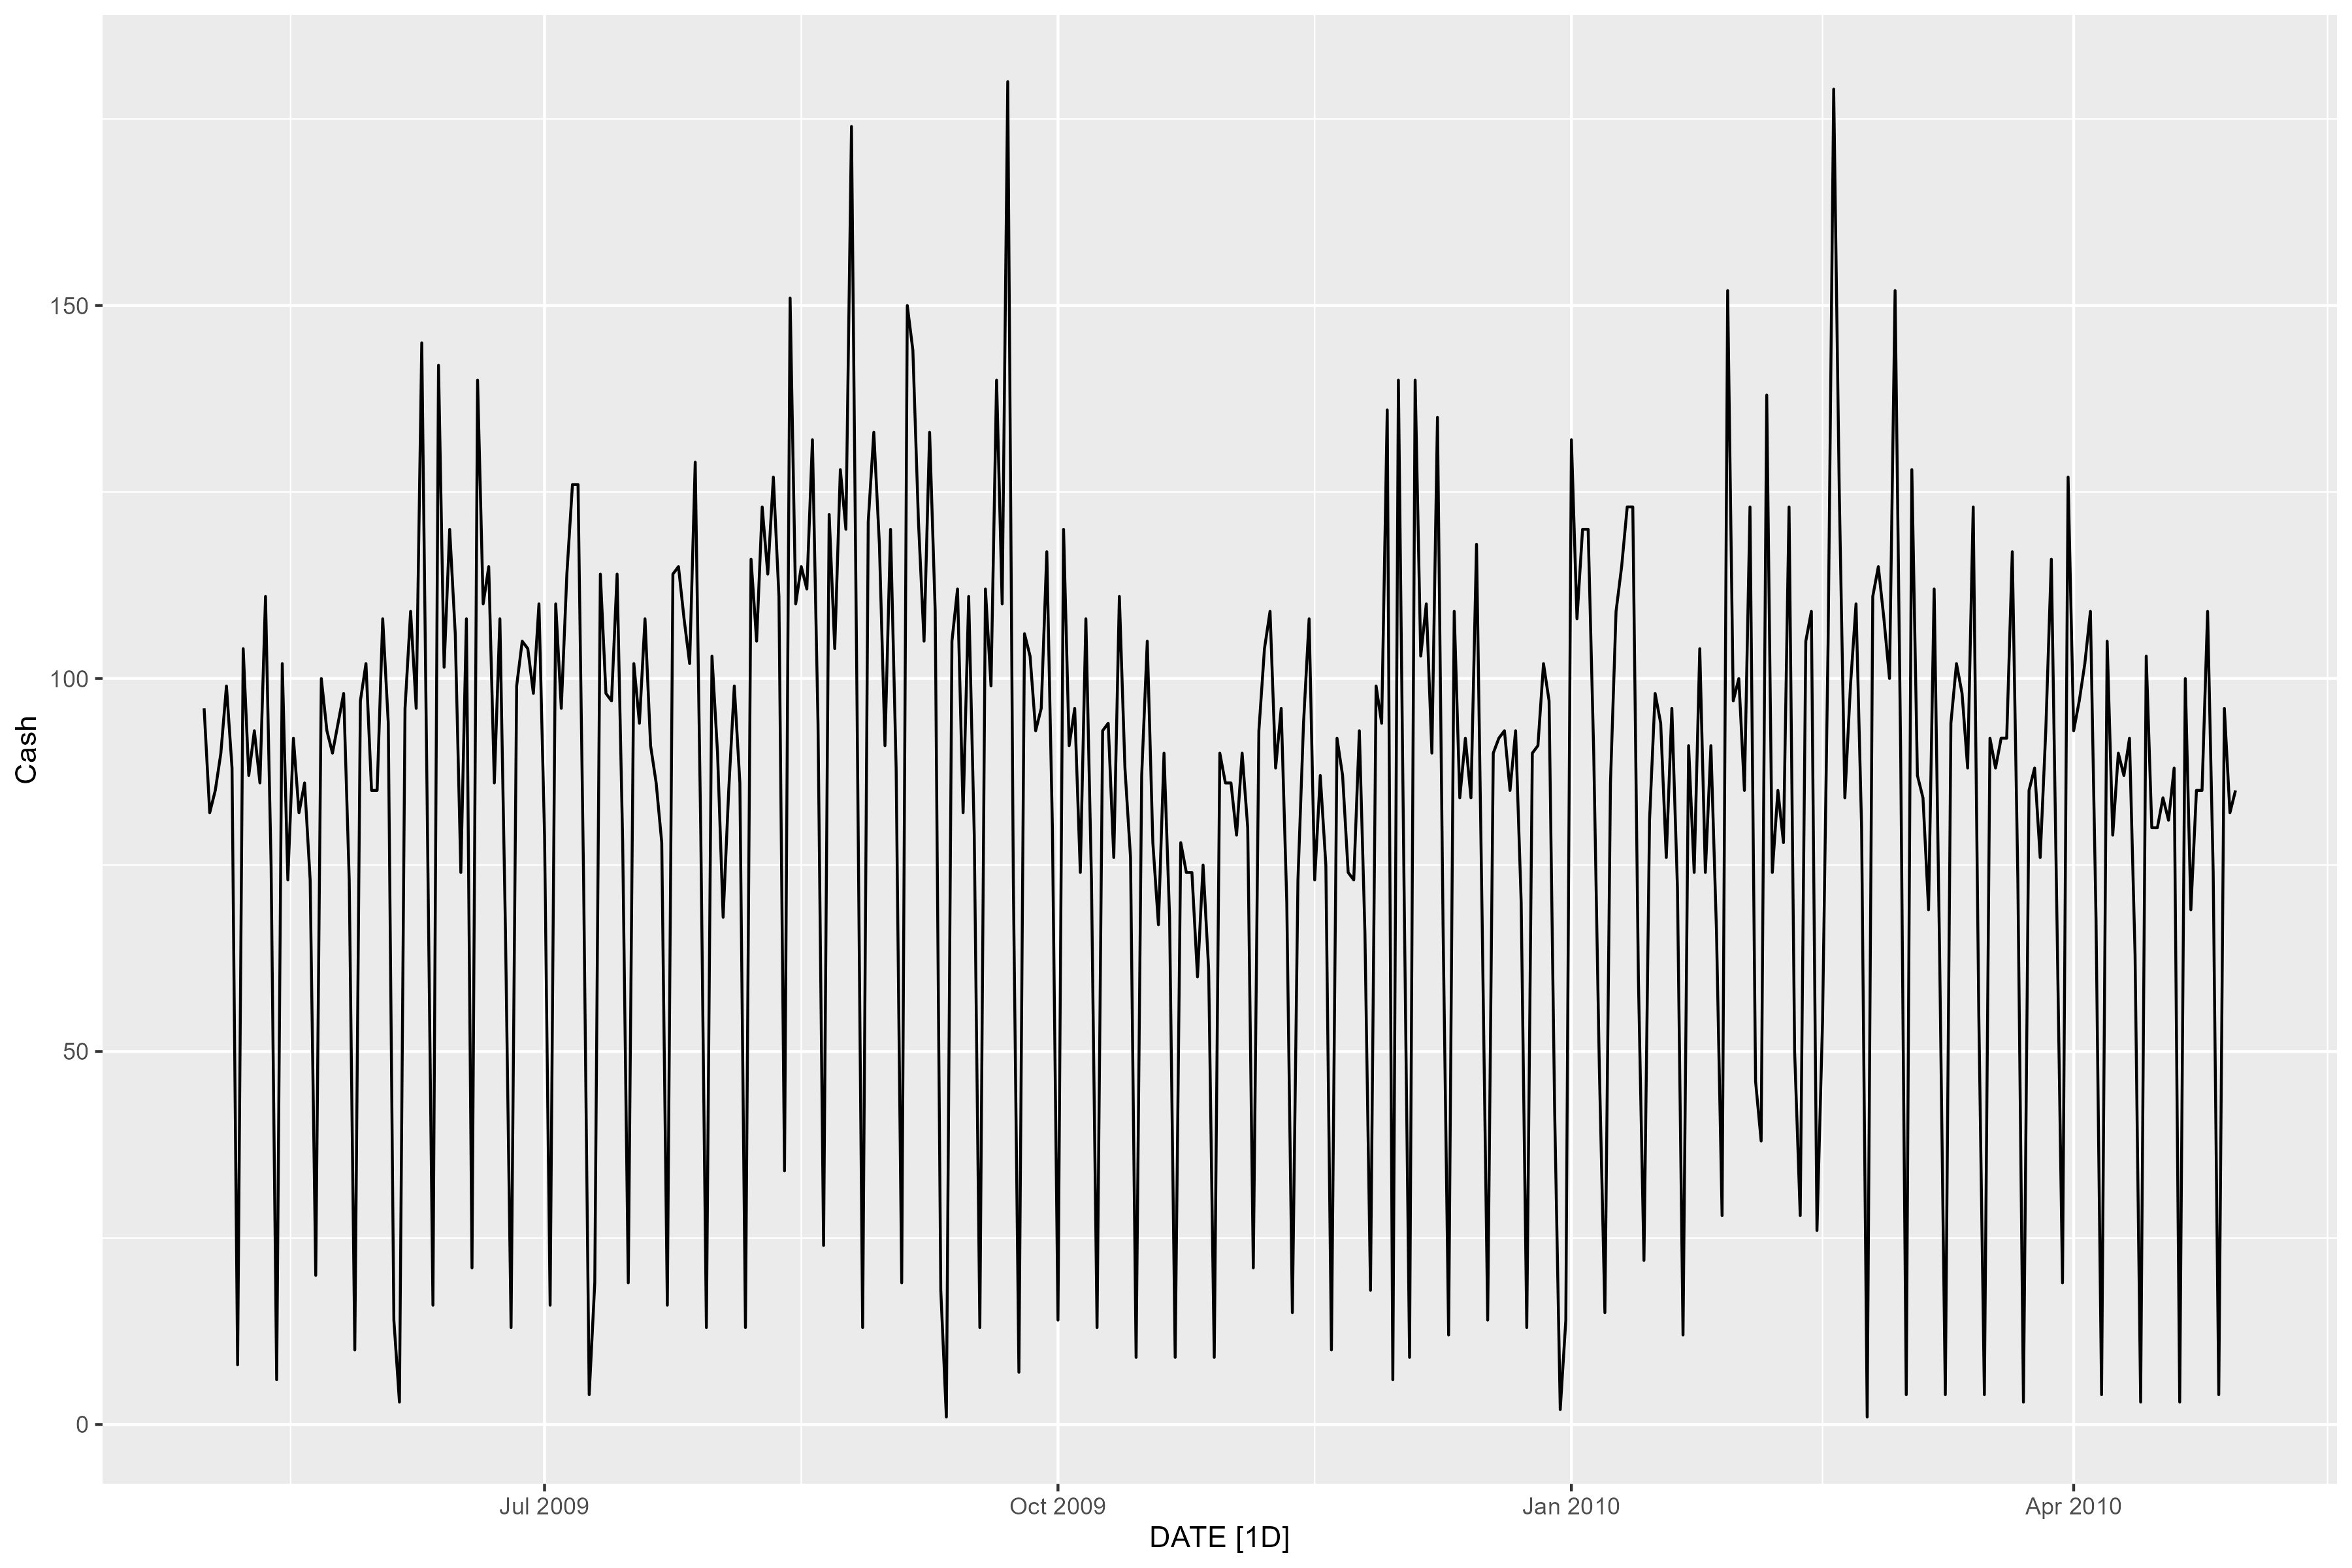
\includegraphics[keepaspectratio]{'images/raw_atm1.png'}}
\caption{Raw ATM1 Plot}
\end{figure}

\textbf{- ATM2}
\pandocbounded{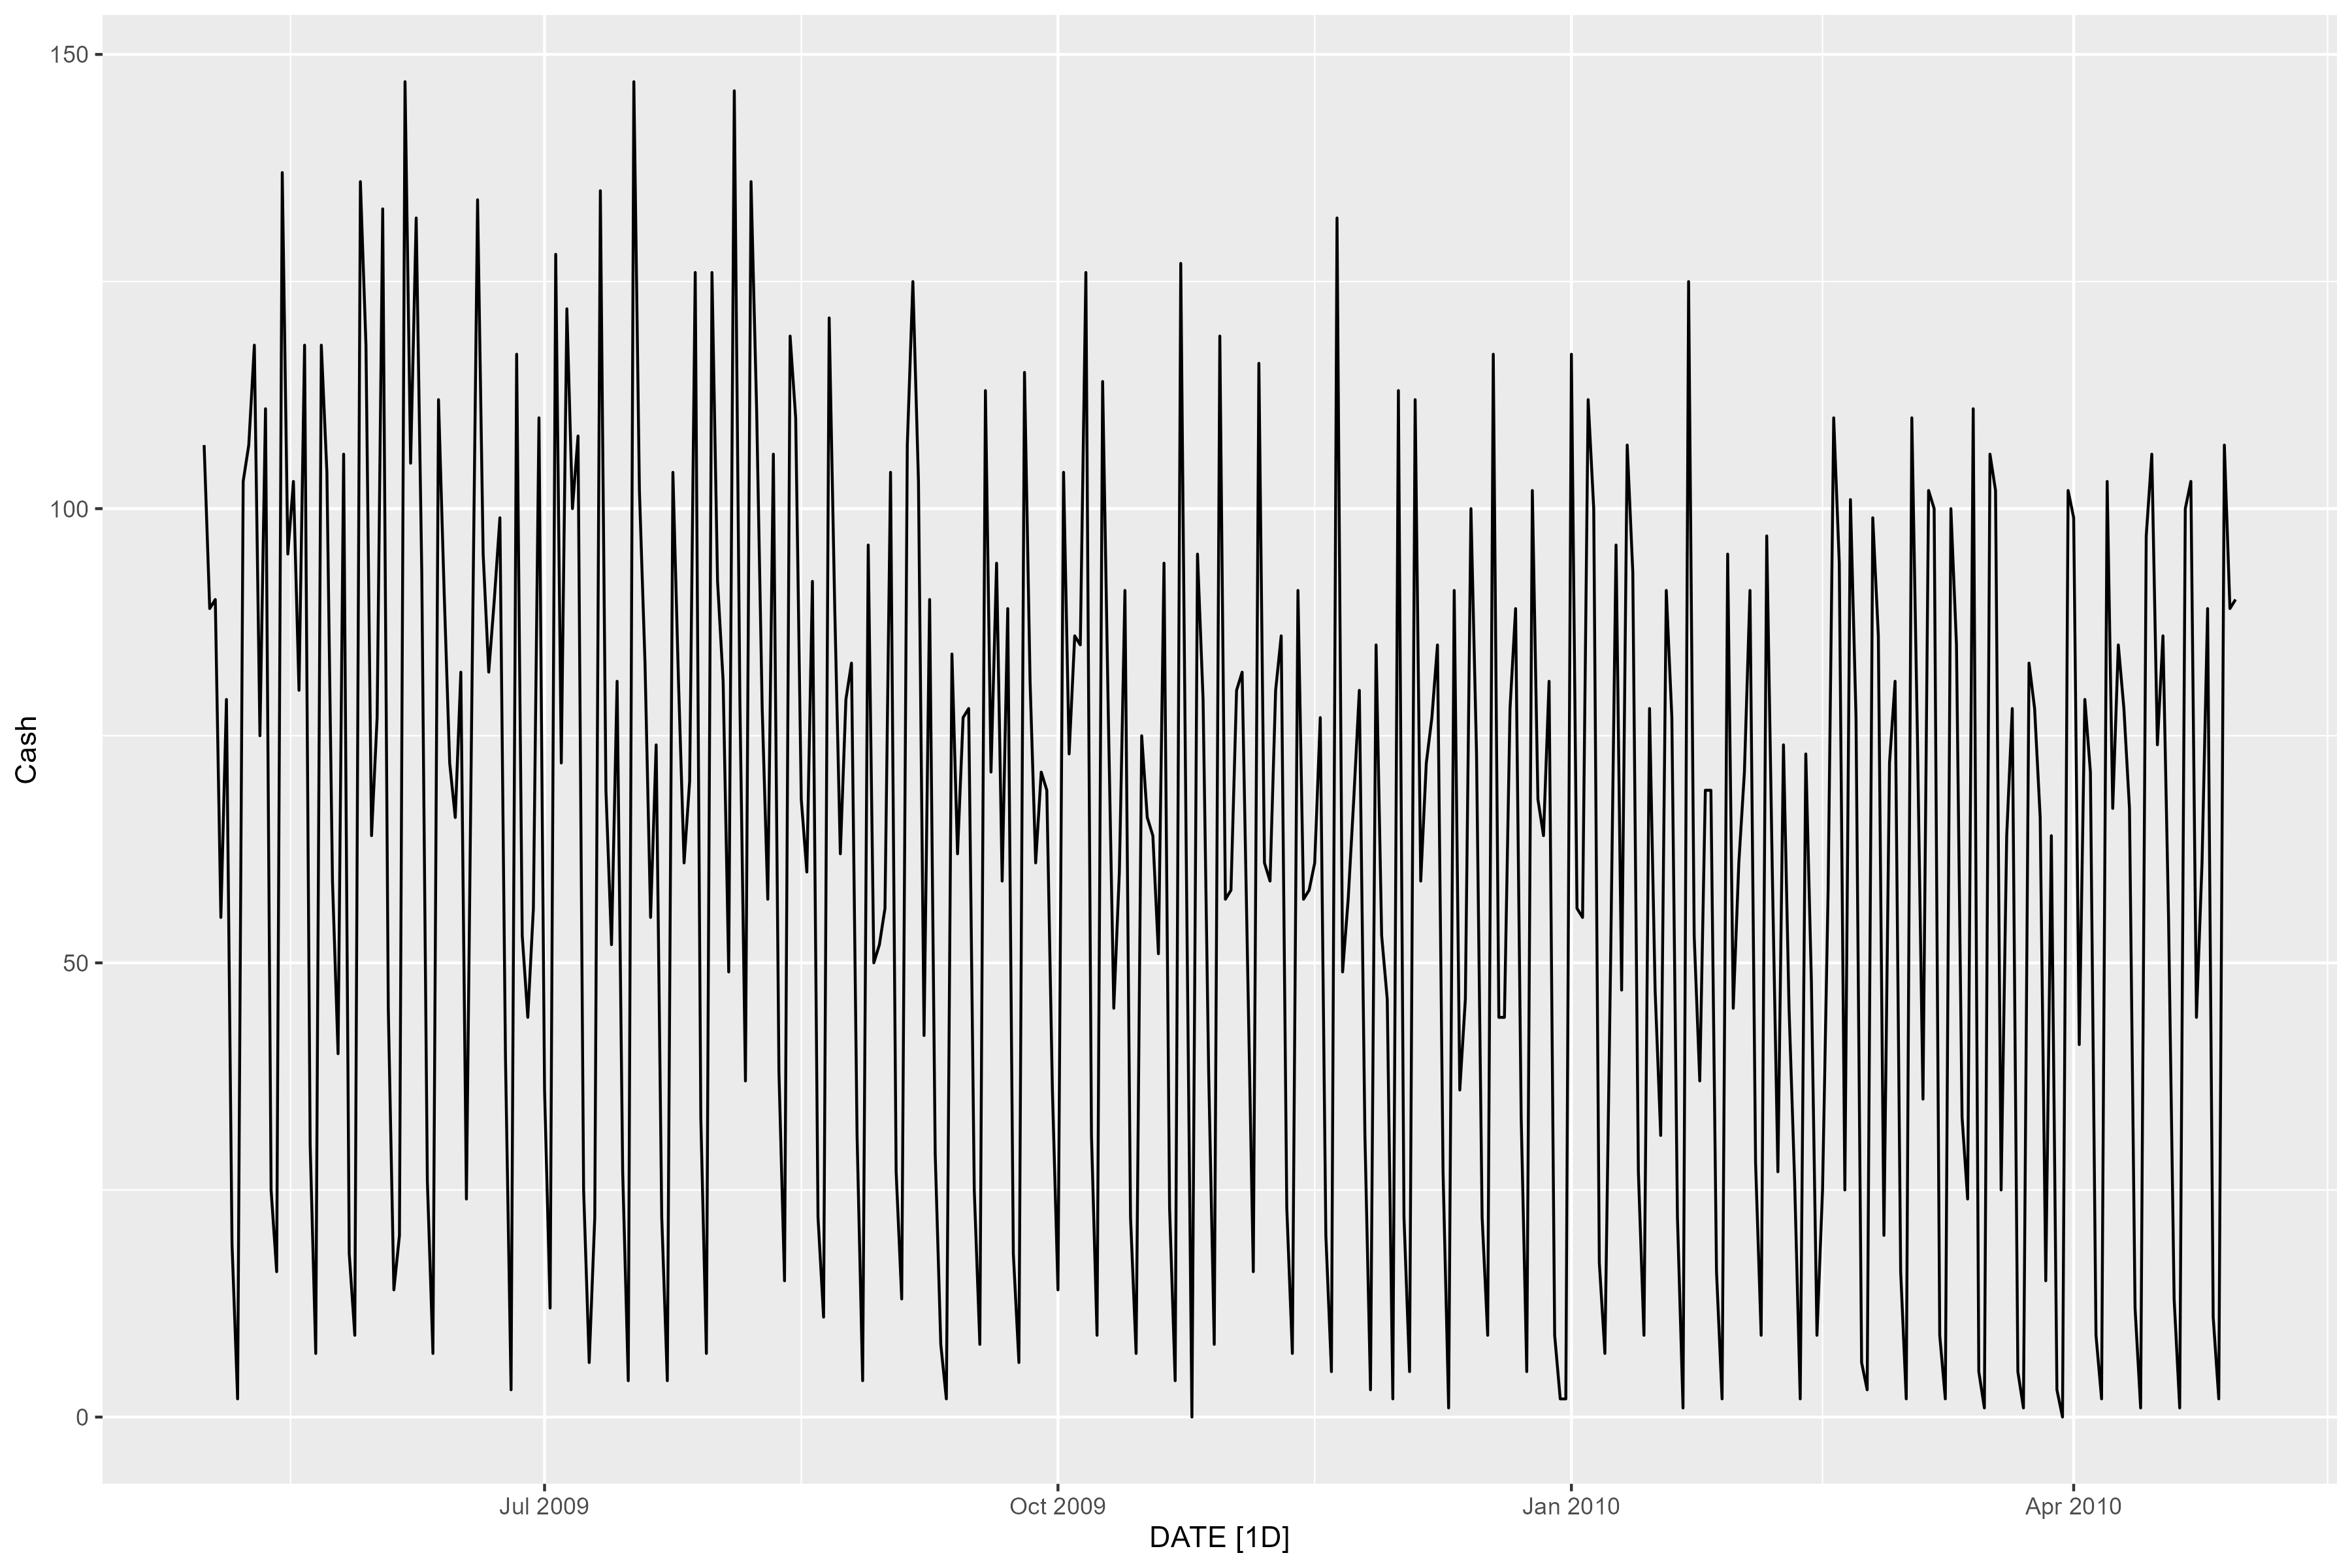
\includegraphics[keepaspectratio]{'images/raw_atm2.png'}}

\textbf{- ATM3}
\pandocbounded{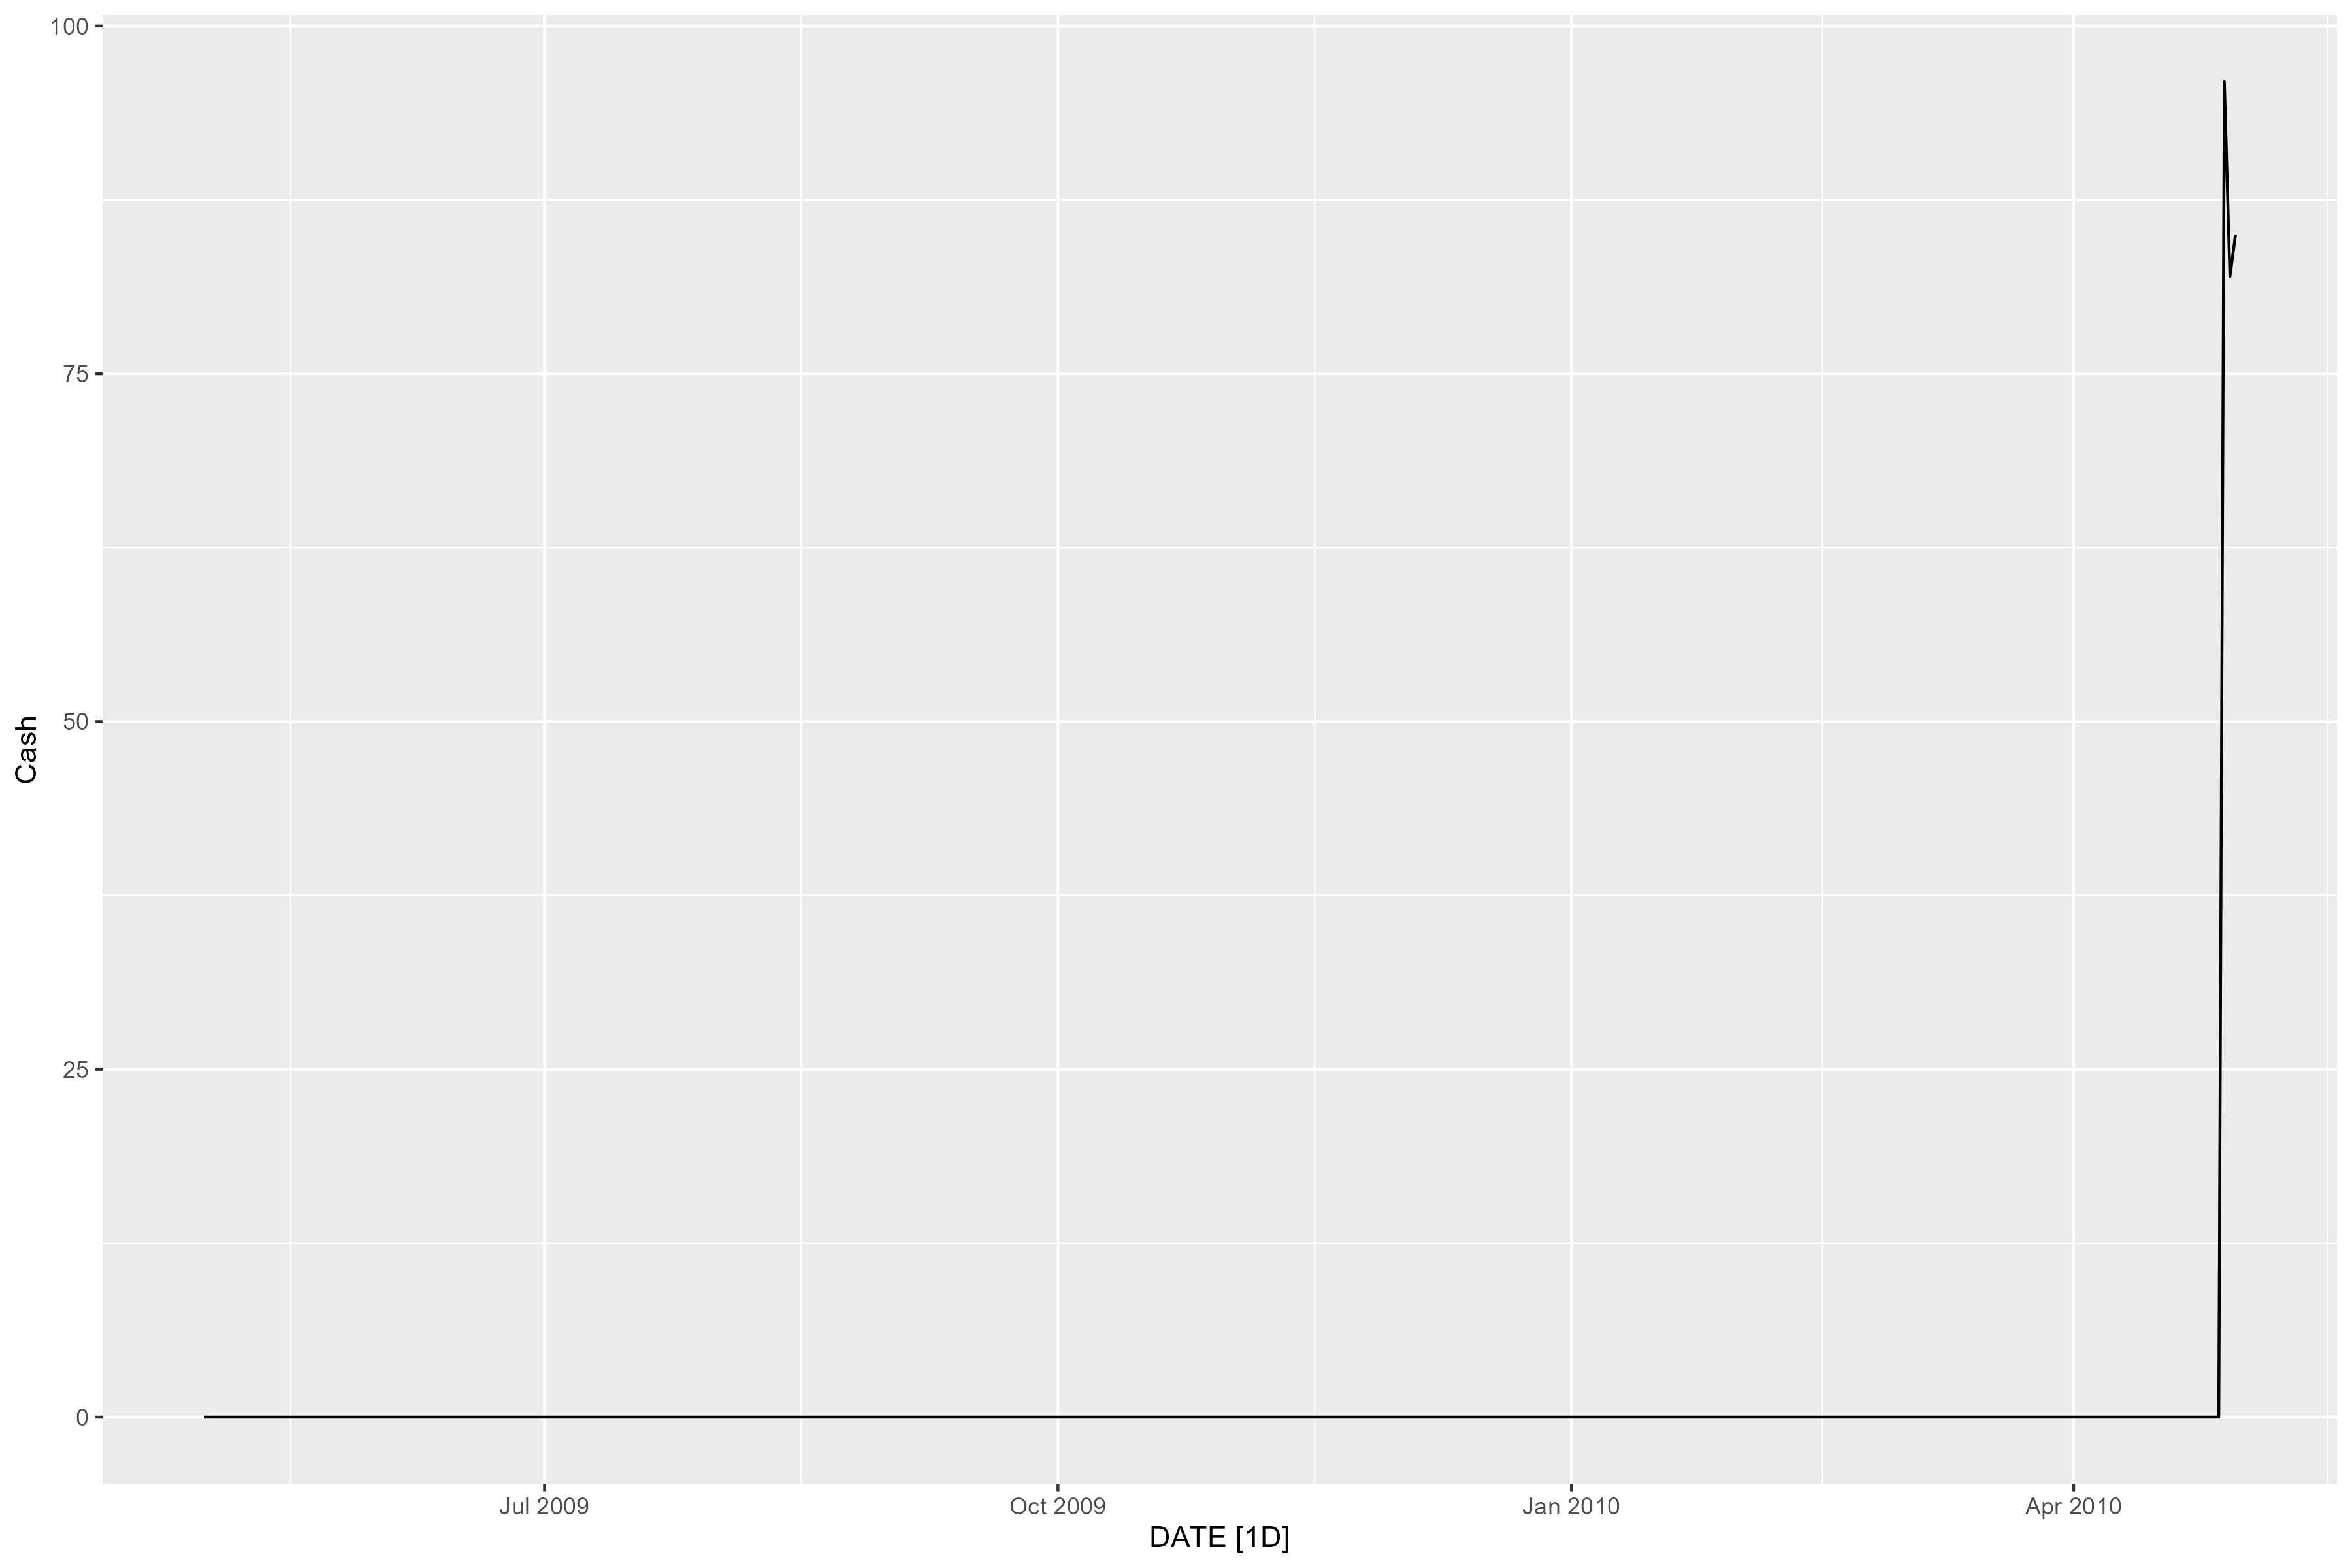
\includegraphics[keepaspectratio]{'images/raw_atm3.png'}}

\begin{figure}
\centering
\pandocbounded{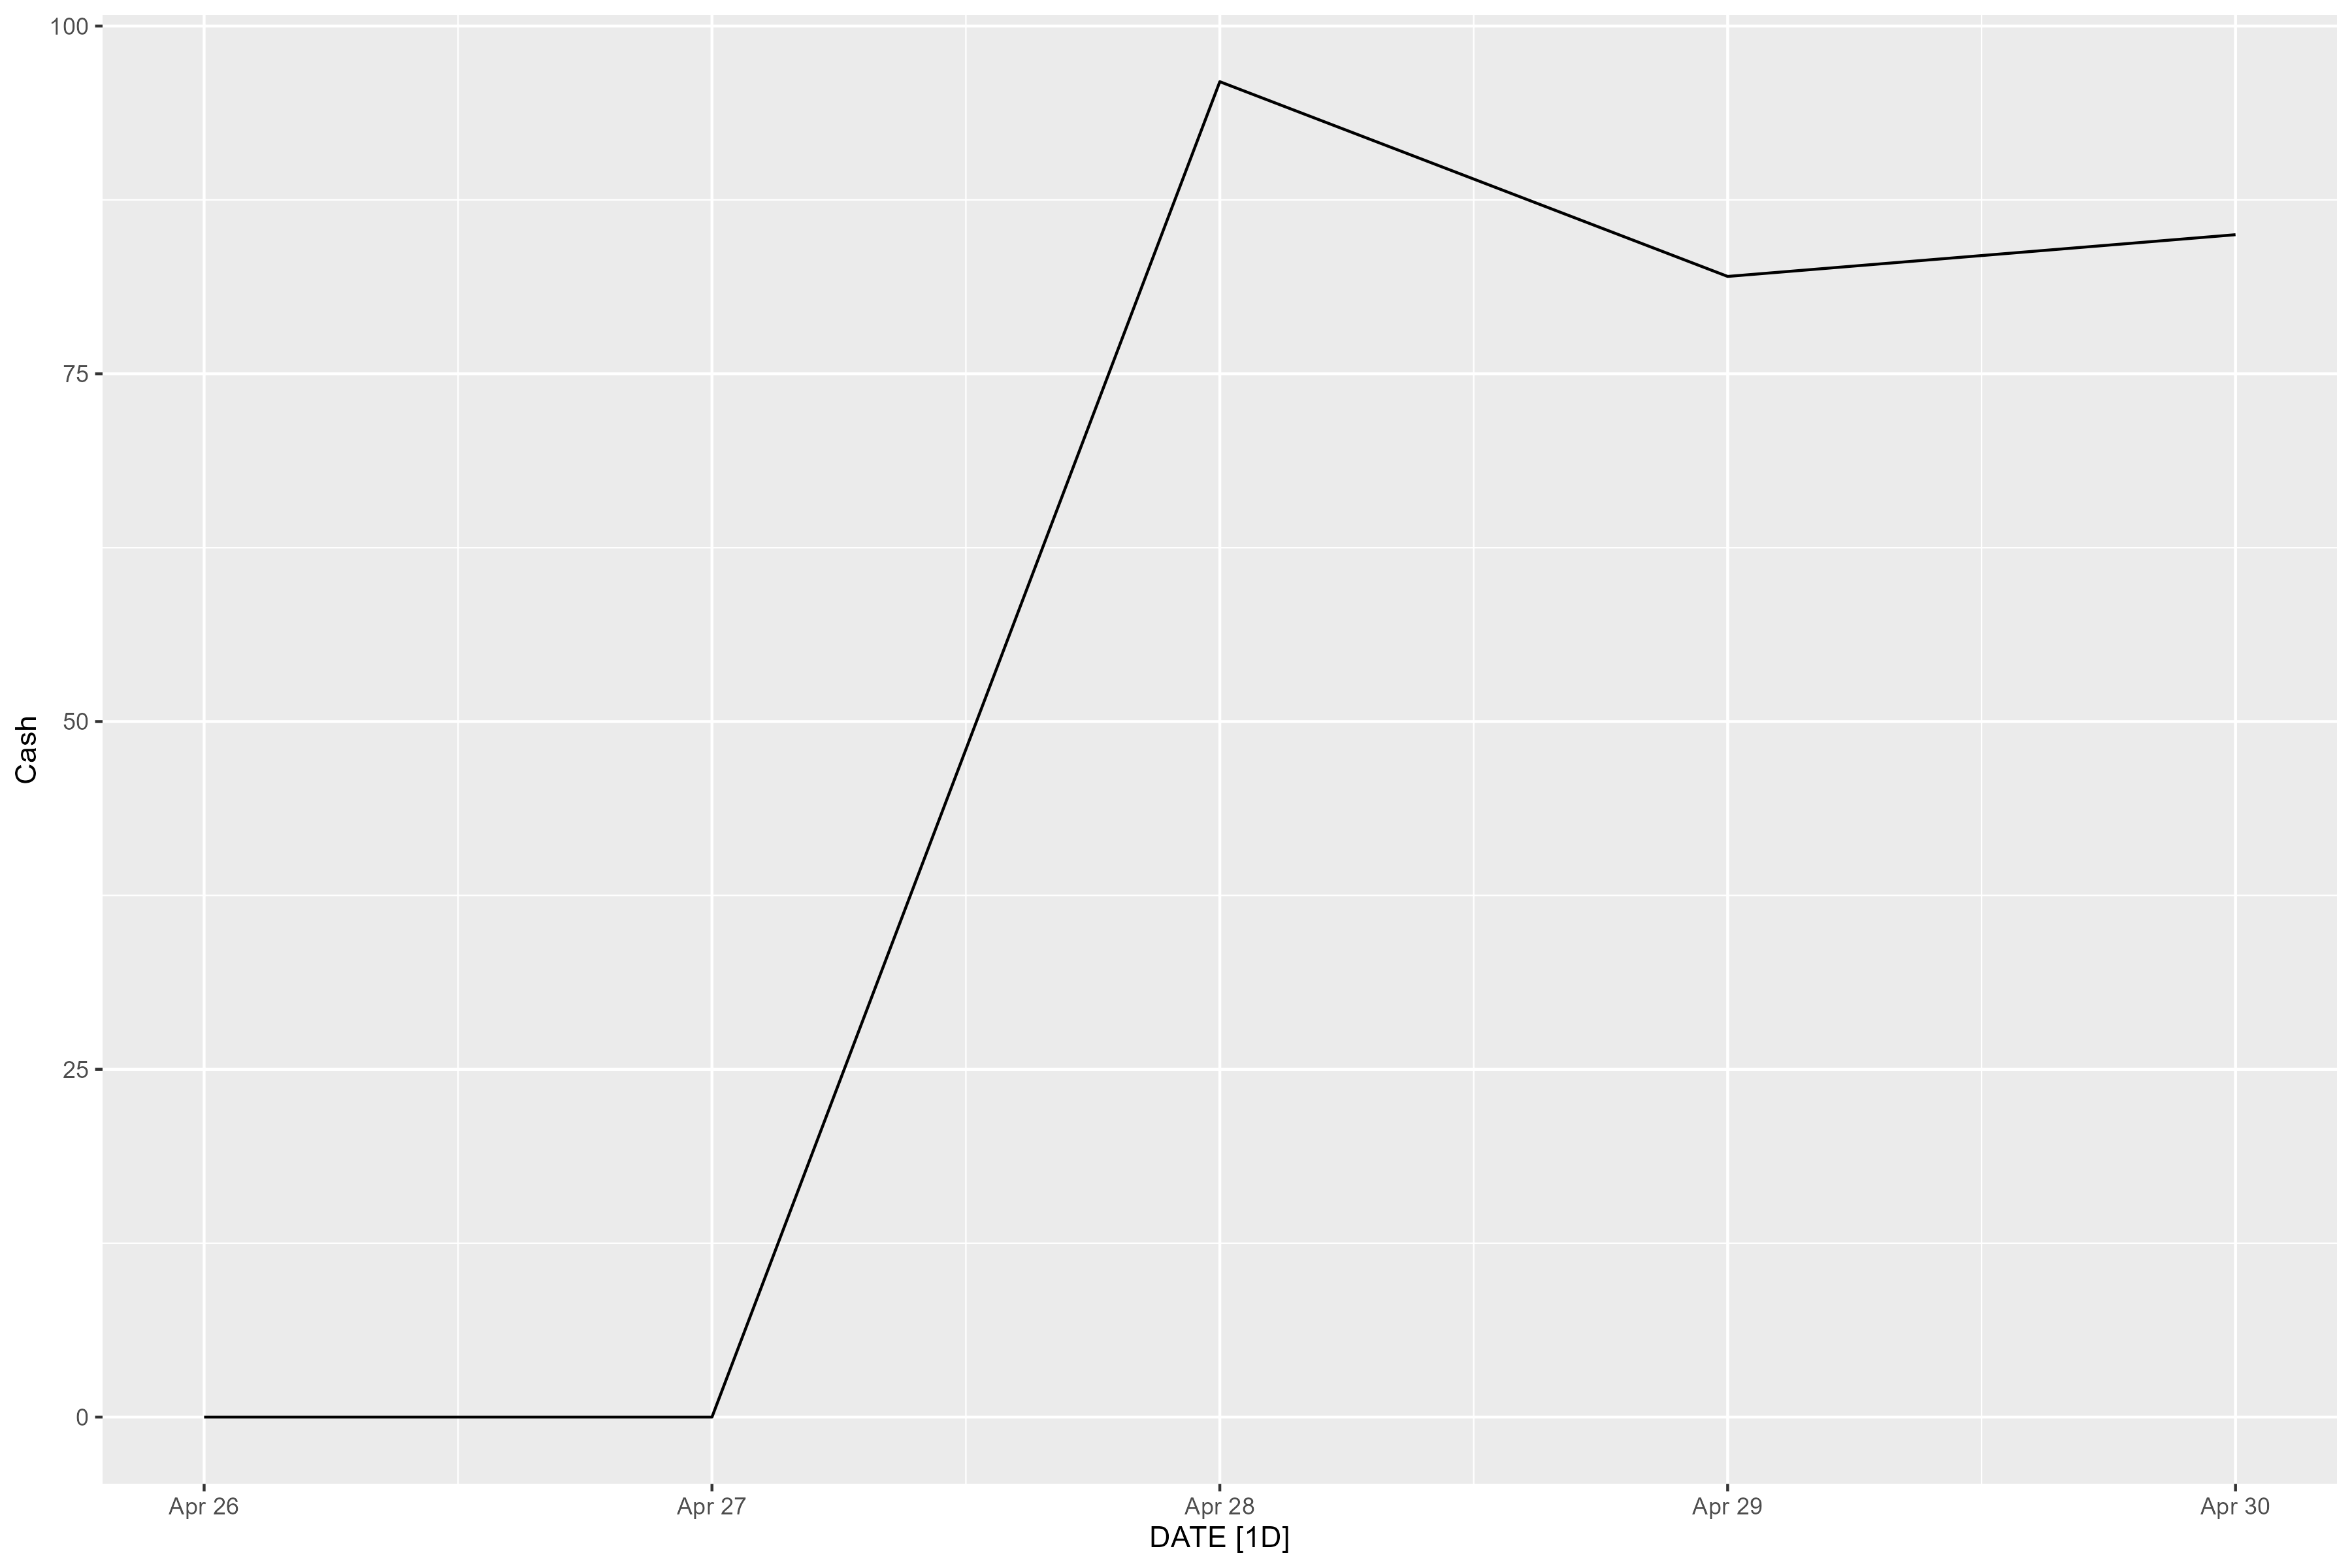
\includegraphics[keepaspectratio]{'images/raw_atm3_lim.png'}}
\caption{Raw ATM3 Plot Limted for Visualization}
\end{figure}

\textbf{- ATM4}
\pandocbounded{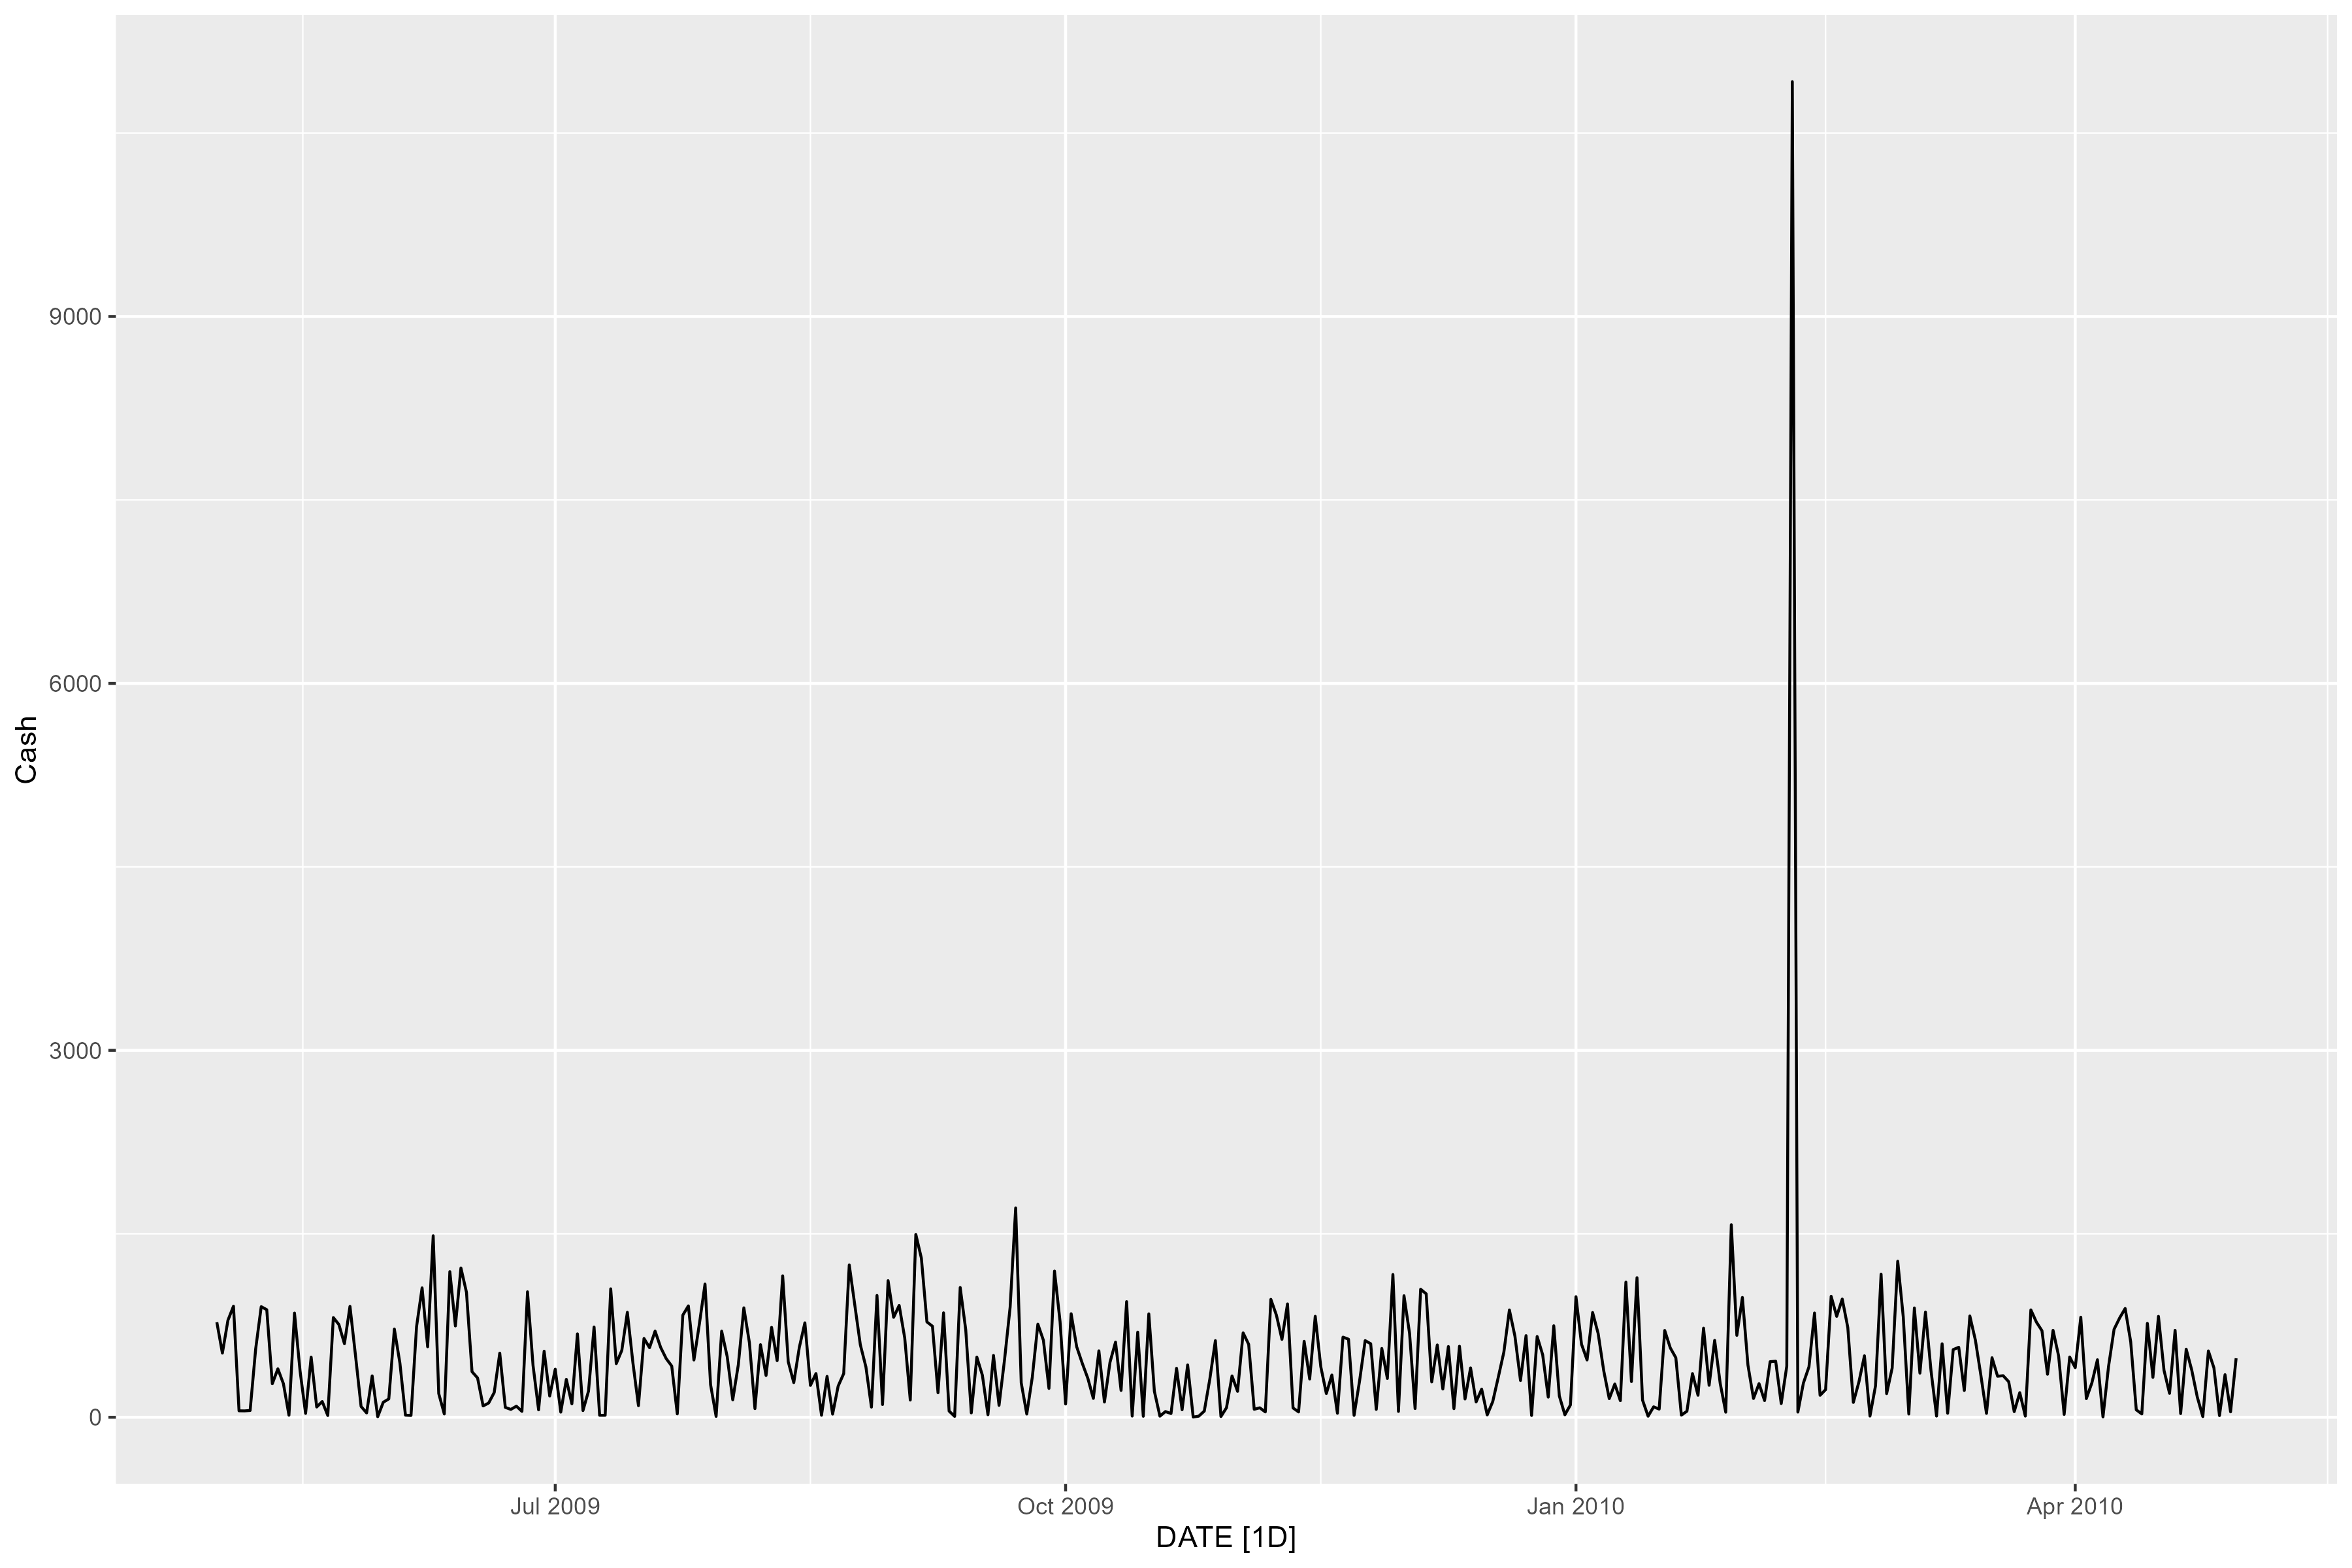
\includegraphics[keepaspectratio]{'images/raw_atm4.png'}}

\paragraph{Code \& Analysis}\label{code-analysis}

\begin{Shaded}
\begin{Highlighting}[]
\CommentTok{\# RAW FILE ALSO SITS HERE: https://raw.githubusercontent.com/jhnboyy/CUNY\_SPS\_WORK/main/Spring2025/DATA624/Project1/ATM624Data.xlsx}
\CommentTok{\#Reading in from local excel }
\NormalTok{atm\_data }\OtherTok{\textless{}{-}} \FunctionTok{read\_excel}\NormalTok{(}\StringTok{"ATM624Data.xlsx"}\NormalTok{)}
\FunctionTok{print}\NormalTok{(}\FunctionTok{head}\NormalTok{(atm\_data))}
\end{Highlighting}
\end{Shaded}

\begin{verbatim}
## # A tibble: 6 x 3
##    DATE ATM    Cash
##   <dbl> <chr> <dbl>
## 1 39934 ATM1     96
## 2 39934 ATM2    107
## 3 39935 ATM1     82
## 4 39935 ATM2     89
## 5 39936 ATM1     85
## 6 39936 ATM2     90
\end{verbatim}

\begin{Shaded}
\begin{Highlighting}[]
\FunctionTok{print}\NormalTok{(}\FunctionTok{nrow}\NormalTok{(atm\_data))}
\end{Highlighting}
\end{Shaded}

\begin{verbatim}
## [1] 1474
\end{verbatim}

\begin{Shaded}
\begin{Highlighting}[]
\DocumentationTok{\#\# initial Processing notes:}
\CommentTok{\# {-} Need to handle date, convert to actual date}
\CommentTok{\# {-} Need to ensure the data is a time series. }
\end{Highlighting}
\end{Shaded}

\begin{Shaded}
\begin{Highlighting}[]
\DocumentationTok{\#\# Checking for nulls and other issues.}
\FunctionTok{print}\NormalTok{(}\FunctionTok{summary}\NormalTok{(atm\_data))}
\end{Highlighting}
\end{Shaded}

\begin{verbatim}
##       DATE           ATM                 Cash        
##  Min.   :39934   Length:1474        Min.   :    0.0  
##  1st Qu.:40026   Class :character   1st Qu.:    0.5  
##  Median :40118   Mode  :character   Median :   73.0  
##  Mean   :40118                      Mean   :  155.6  
##  3rd Qu.:40210                      3rd Qu.:  114.0  
##  Max.   :40312                      Max.   :10919.8  
##                                     NA's   :19
\end{verbatim}

\begin{Shaded}
\begin{Highlighting}[]
\DocumentationTok{\#\# The cash category has 19 nulls.}
\DocumentationTok{\#\# Min of 0 max of 10,919. Mean of 155. }
\DocumentationTok{\#\# Data has no nulls, right now is listed as number. }
\DocumentationTok{\#\# ATM is character, non numeric. Looking at unique vals.}

\FunctionTok{print}\NormalTok{(}\FunctionTok{unique}\NormalTok{(atm\_data}\SpecialCharTok{$}\NormalTok{ATM))}
\end{Highlighting}
\end{Shaded}

\begin{verbatim}
## [1] "ATM1" "ATM2" NA     "ATM3" "ATM4"
\end{verbatim}

\begin{Shaded}
\begin{Highlighting}[]
\CommentTok{\# There is an \textquotesingle{}NA\textquotesingle{} Value here lets take a look}

\NormalTok{atm\_null }\OtherTok{\textless{}{-}}\NormalTok{ atm\_data }\SpecialCharTok{|\textgreater{}} \FunctionTok{filter}\NormalTok{(}\FunctionTok{is.na}\NormalTok{(ATM))}

\FunctionTok{print}\NormalTok{(}\FunctionTok{nrow}\NormalTok{(atm\_null))}
\end{Highlighting}
\end{Shaded}

\begin{verbatim}
## [1] 14
\end{verbatim}

\begin{Shaded}
\begin{Highlighting}[]
\CommentTok{\# 14 rows where ATM is null.}

\FunctionTok{print}\NormalTok{(}\FunctionTok{unique}\NormalTok{(atm\_null}\SpecialCharTok{$}\NormalTok{Cash))}
\end{Highlighting}
\end{Shaded}

\begin{verbatim}
## [1] NA
\end{verbatim}

\begin{Shaded}
\begin{Highlighting}[]
\CommentTok{\# All Cash values are null for where the ATM column is null. These Rows should just be removed? }

\DocumentationTok{\#\# Looking at the additional Cash values that are null with ATM values.}
\NormalTok{atm\_data }\SpecialCharTok{|\textgreater{}} \FunctionTok{filter}\NormalTok{(}\SpecialCharTok{!}\FunctionTok{is.na}\NormalTok{(ATM), }\FunctionTok{is.na}\NormalTok{(Cash))}
\end{Highlighting}
\end{Shaded}

\begin{verbatim}
## # A tibble: 5 x 3
##    DATE ATM    Cash
##   <dbl> <chr> <dbl>
## 1 39977 ATM1     NA
## 2 39980 ATM1     NA
## 3 39982 ATM2     NA
## 4 39986 ATM1     NA
## 5 39988 ATM2     NA
\end{verbatim}

\begin{Shaded}
\begin{Highlighting}[]
\DocumentationTok{\#\# Cash Nulls with ATM values are limited to ATM 1 and ATM 2. We should impute these 4 rows. }

\CommentTok{\# Dropping the ATM\_Nulls}
\NormalTok{atm\_data }\OtherTok{\textless{}{-}}\NormalTok{ atm\_data }\SpecialCharTok{|\textgreater{}} \FunctionTok{filter}\NormalTok{(}\SpecialCharTok{!}\FunctionTok{is.na}\NormalTok{(ATM))}
\end{Highlighting}
\end{Shaded}

\begin{Shaded}
\begin{Highlighting}[]
\DocumentationTok{\#\# After manually reviwing the data in excel data "DATE" column is actually a time stamp. However, its at midnight for each day so i think a date is good enough. }
\DocumentationTok{\#\# Also had to google how excel does dates for the origin date. Evidently excel incorrectly treats 1900 as a leap year when it wasnt. (INSANE!)}
\DocumentationTok{\#\# So need to use 1899}
\CommentTok{\#(Srouce: https://community.alteryx.com/t5/Alteryx{-}Designer{-}Desktop{-}Discussions/Rounding{-}DateTime{-}error{-}when{-}Importing{-}Excel/td{-}p/592023)}
\NormalTok{atm\_data }\OtherTok{\textless{}{-}}\NormalTok{atm\_data }\SpecialCharTok{|\textgreater{}} \FunctionTok{mutate}\NormalTok{(}\AttributeTok{DATE =} \FunctionTok{as.Date}\NormalTok{(DATE,}\AttributeTok{origin =} \StringTok{"1899{-}12{-}30"}\NormalTok{))}

\CommentTok{\# Null Cash Imputation}
\CommentTok{\#atm\_data |\textgreater{} filter(is.na(Cash))}

\DocumentationTok{\#\# Adding A column to Keep tabs on imputations}
\NormalTok{atm\_data }\OtherTok{\textless{}{-}}\NormalTok{ atm\_data }\SpecialCharTok{|\textgreater{}}\FunctionTok{mutate}\NormalTok{(}\AttributeTok{source =} \FunctionTok{if\_else}\NormalTok{(}\FunctionTok{is.na}\NormalTok{(Cash), }\StringTok{"imputed"}\NormalTok{, }\StringTok{"original"}\NormalTok{))}

\DocumentationTok{\#\# Firstly Dealing with ATM 1 nulls }
\NormalTok{atm\_data }\SpecialCharTok{|\textgreater{}} \FunctionTok{filter}\NormalTok{(}\FunctionTok{is.na}\NormalTok{(Cash), ATM }\SpecialCharTok{==}\StringTok{\textquotesingle{}ATM1\textquotesingle{}}\NormalTok{)}
\end{Highlighting}
\end{Shaded}

\begin{verbatim}
## # A tibble: 3 x 4
##   DATE       ATM    Cash source 
##   <date>     <chr> <dbl> <chr>  
## 1 2009-06-13 ATM1     NA imputed
## 2 2009-06-16 ATM1     NA imputed
## 3 2009-06-22 ATM1     NA imputed
\end{verbatim}

\begin{Shaded}
\begin{Highlighting}[]
\CommentTok{\# The nulls are limited 6/13/2009, 6/16/2009, 06/22/2009}

\DocumentationTok{\#\# Checking the data for dates in this month for ATM1}
\NormalTok{atm\_data }\SpecialCharTok{|\textgreater{}} \FunctionTok{filter}\NormalTok{(DATE}\SpecialCharTok{\textgreater{}}\StringTok{\textquotesingle{}2009{-}06{-}11\textquotesingle{}}\NormalTok{,DATE}\SpecialCharTok{\textless{}}\StringTok{\textquotesingle{}2009{-}06{-}25\textquotesingle{}}\NormalTok{ , ATM }\SpecialCharTok{==}\StringTok{\textquotesingle{}ATM1\textquotesingle{}}\NormalTok{)}
\end{Highlighting}
\end{Shaded}

\begin{verbatim}
## # A tibble: 13 x 4
##    DATE       ATM    Cash source  
##    <date>     <chr> <dbl> <chr>   
##  1 2009-06-12 ATM1    142 original
##  2 2009-06-13 ATM1     NA imputed 
##  3 2009-06-14 ATM1    120 original
##  4 2009-06-15 ATM1    106 original
##  5 2009-06-16 ATM1     NA imputed 
##  6 2009-06-17 ATM1    108 original
##  7 2009-06-18 ATM1     21 original
##  8 2009-06-19 ATM1    140 original
##  9 2009-06-20 ATM1    110 original
## 10 2009-06-21 ATM1    115 original
## 11 2009-06-22 ATM1     NA imputed 
## 12 2009-06-23 ATM1    108 original
## 13 2009-06-24 ATM1     66 original
\end{verbatim}

\begin{Shaded}
\begin{Highlighting}[]
\DocumentationTok{\#\# For ATM 1 there are values sandwiching each of the missing values so were going to just take the average of the "bookend" dates for each missing value. Its only 3 values.}
\CommentTok{\#atm\_data |\textgreater{} filter(DATE\textgreater{}\textquotesingle{}2009{-}06{-}11\textquotesingle{},DATE\textless{}\textquotesingle{}2009{-}06{-}15\textquotesingle{} , ATM ==\textquotesingle{}ATM1\textquotesingle{}) |\textgreater{} mutate()}

\NormalTok{atm\_data\_imputed }\OtherTok{\textless{}{-}}\NormalTok{ atm\_data }\SpecialCharTok{|\textgreater{}} \FunctionTok{mutate}\NormalTok{(}\AttributeTok{Cash =} \FunctionTok{if\_else}\NormalTok{(}\FunctionTok{is.na}\NormalTok{(Cash) }\SpecialCharTok{\&}\NormalTok{ ATM }\SpecialCharTok{==} \StringTok{"ATM1"} \SpecialCharTok{\&}\NormalTok{ DATE }\SpecialCharTok{\textgreater{}} \FunctionTok{as.Date}\NormalTok{(}\StringTok{"2009{-}06{-}11"}\NormalTok{) }\SpecialCharTok{\&}\NormalTok{ DATE }\SpecialCharTok{\textless{}} \FunctionTok{as.Date}\NormalTok{(}\StringTok{"2009{-}06{-}15"}\NormalTok{),}
\NormalTok{                                  (}\FunctionTok{lag}\NormalTok{(Cash) }\SpecialCharTok{+} \FunctionTok{lead}\NormalTok{(Cash)) }\SpecialCharTok{/} \DecValTok{2}\NormalTok{, Cash ))}
\CommentTok{\#Confirming}
\CommentTok{\#atm\_data\_imputed |\textgreater{} filter(DATE\textgreater{}\textquotesingle{}2009{-}06{-}11\textquotesingle{},DATE\textless{}\textquotesingle{}2009{-}06{-}15\textquotesingle{} , ATM ==\textquotesingle{}ATM1\textquotesingle{})}

\DocumentationTok{\#\# Dealing with 6/16/2009 Null}
\CommentTok{\#atm\_data\_imputed |\textgreater{} filter(DATE\textgreater{}\textquotesingle{}2009{-}06{-}14\textquotesingle{},DATE\textless{}\textquotesingle{}2009{-}06{-}18\textquotesingle{} , ATM ==\textquotesingle{}ATM1\textquotesingle{})}
\NormalTok{atm\_data\_imputed }\OtherTok{\textless{}{-}}\NormalTok{ atm\_data\_imputed }\SpecialCharTok{|\textgreater{}} \FunctionTok{mutate}\NormalTok{(}\AttributeTok{Cash =} \FunctionTok{if\_else}\NormalTok{(}\FunctionTok{is.na}\NormalTok{(Cash) }\SpecialCharTok{\&}\NormalTok{ ATM }\SpecialCharTok{==} \StringTok{"ATM1"} \SpecialCharTok{\&}\NormalTok{ DATE }\SpecialCharTok{\textgreater{}} \FunctionTok{as.Date}\NormalTok{(}\StringTok{"2009{-}06{-}14"}\NormalTok{) }\SpecialCharTok{\&}\NormalTok{ DATE }\SpecialCharTok{\textless{}} \FunctionTok{as.Date}\NormalTok{(}\StringTok{"2009{-}06{-}18"}\NormalTok{),}
\NormalTok{                                  (}\FunctionTok{lag}\NormalTok{(Cash) }\SpecialCharTok{+} \FunctionTok{lead}\NormalTok{(Cash)) }\SpecialCharTok{/} \DecValTok{2}\NormalTok{, Cash ))}
\CommentTok{\#Confirming}
\CommentTok{\#atm\_data\_imputed |\textgreater{} filter(DATE\textgreater{}\textquotesingle{}2009{-}06{-}14\textquotesingle{},DATE\textless{}\textquotesingle{}2009{-}06{-}18\textquotesingle{} , ATM ==\textquotesingle{}ATM1\textquotesingle{})}

\CommentTok{\# Dealing with the 06/22/2009}
\NormalTok{atm\_data\_imputed }\OtherTok{\textless{}{-}}\NormalTok{ atm\_data\_imputed }\SpecialCharTok{|\textgreater{}} \FunctionTok{mutate}\NormalTok{(}\AttributeTok{Cash =} \FunctionTok{if\_else}\NormalTok{(}\FunctionTok{is.na}\NormalTok{(Cash) }\SpecialCharTok{\&}\NormalTok{ ATM }\SpecialCharTok{==} \StringTok{"ATM1"} \SpecialCharTok{\&}\NormalTok{ DATE }\SpecialCharTok{\textgreater{}} \FunctionTok{as.Date}\NormalTok{(}\StringTok{"2009{-}06{-}20"}\NormalTok{) }\SpecialCharTok{\&}\NormalTok{ DATE }\SpecialCharTok{\textless{}} \FunctionTok{as.Date}\NormalTok{(}\StringTok{"2009{-}06{-}24"}\NormalTok{),}
\NormalTok{                                  (}\FunctionTok{lag}\NormalTok{(Cash) }\SpecialCharTok{+} \FunctionTok{lead}\NormalTok{(Cash)) }\SpecialCharTok{/} \DecValTok{2}\NormalTok{, Cash ))}

\CommentTok{\#atm\_data\_imputed |\textgreater{} filter(DATE\textgreater{}\textquotesingle{}2009{-}06{-}20\textquotesingle{},DATE\textless{}\textquotesingle{}2009{-}06{-}24\textquotesingle{} , ATM ==\textquotesingle{}ATM1\textquotesingle{})}

\DocumentationTok{\#\# FINISHED WITH ATM 1 NULLS, MOVING TO ATM2 NULLS}
\NormalTok{atm\_data\_imputed }\SpecialCharTok{|\textgreater{}} \FunctionTok{filter}\NormalTok{(}\FunctionTok{is.na}\NormalTok{(Cash), ATM }\SpecialCharTok{==}\StringTok{\textquotesingle{}ATM2\textquotesingle{}}\NormalTok{)}
\end{Highlighting}
\end{Shaded}

\begin{verbatim}
## # A tibble: 2 x 4
##   DATE       ATM    Cash source 
##   <date>     <chr> <dbl> <chr>  
## 1 2009-06-18 ATM2     NA imputed
## 2 2009-06-24 ATM2     NA imputed
\end{verbatim}

\begin{Shaded}
\begin{Highlighting}[]
\DocumentationTok{\#\# ATM 2 Nulls are limited to 06/18/2009 and 06/24/2009}

\DocumentationTok{\#\# First instance at 6/18/2009}
\CommentTok{\#atm\_data\_imputed |\textgreater{} filter(DATE\textgreater{}\textquotesingle{}2009{-}06{-}16\textquotesingle{},DATE\textless{}\textquotesingle{}2009{-}06{-}20\textquotesingle{} , ATM ==\textquotesingle{}ATM2\textquotesingle{})}
\NormalTok{atm\_data\_imputed }\OtherTok{\textless{}{-}}\NormalTok{ atm\_data\_imputed }\SpecialCharTok{|\textgreater{}} \FunctionTok{mutate}\NormalTok{(}\AttributeTok{Cash =} \FunctionTok{if\_else}\NormalTok{(}\FunctionTok{is.na}\NormalTok{(Cash) }\SpecialCharTok{\&}\NormalTok{ ATM }\SpecialCharTok{==} \StringTok{"ATM2"} \SpecialCharTok{\&}\NormalTok{ DATE }\SpecialCharTok{\textgreater{}} \FunctionTok{as.Date}\NormalTok{(}\StringTok{"2009{-}06{-}16"}\NormalTok{) }\SpecialCharTok{\&}\NormalTok{ DATE }\SpecialCharTok{\textless{}} \FunctionTok{as.Date}\NormalTok{(}\StringTok{"2009{-}06{-}20"}\NormalTok{),}
\NormalTok{                                  (}\FunctionTok{lag}\NormalTok{(Cash) }\SpecialCharTok{+} \FunctionTok{lead}\NormalTok{(Cash)) }\SpecialCharTok{/} \DecValTok{2}\NormalTok{, Cash ))}
\CommentTok{\#Checking}
\CommentTok{\#atm\_data\_imputed |\textgreater{} filter(DATE\textgreater{}\textquotesingle{}2009{-}06{-}16\textquotesingle{},DATE\textless{}\textquotesingle{}2009{-}06{-}20\textquotesingle{} , ATM ==\textquotesingle{}ATM2\textquotesingle{})}

\CommentTok{\# Second instance at 6/24/2009}
\CommentTok{\#atm\_data\_imputed |\textgreater{} filter(DATE\textgreater{}\textquotesingle{}2009{-}06{-}22\textquotesingle{},DATE\textless{}\textquotesingle{}2009{-}06{-}26\textquotesingle{} , ATM ==\textquotesingle{}ATM2\textquotesingle{})}
\NormalTok{atm\_data\_imputed }\OtherTok{\textless{}{-}}\NormalTok{ atm\_data\_imputed }\SpecialCharTok{|\textgreater{}} \FunctionTok{mutate}\NormalTok{(}\AttributeTok{Cash =} \FunctionTok{if\_else}\NormalTok{(}\FunctionTok{is.na}\NormalTok{(Cash) }\SpecialCharTok{\&}\NormalTok{ ATM }\SpecialCharTok{==} \StringTok{"ATM2"} \SpecialCharTok{\&}\NormalTok{ DATE }\SpecialCharTok{\textgreater{}} \FunctionTok{as.Date}\NormalTok{(}\StringTok{"2009{-}06{-}22"}\NormalTok{) }\SpecialCharTok{\&}\NormalTok{ DATE }\SpecialCharTok{\textless{}} \FunctionTok{as.Date}\NormalTok{(}\StringTok{"2009{-}06{-}26"}\NormalTok{),}
\NormalTok{                                  (}\FunctionTok{lag}\NormalTok{(Cash) }\SpecialCharTok{+} \FunctionTok{lead}\NormalTok{(Cash)) }\SpecialCharTok{/} \DecValTok{2}\NormalTok{, Cash ))}
\CommentTok{\#Checking}
\CommentTok{\#atm\_data\_imputed |\textgreater{} filter(DATE\textgreater{}\textquotesingle{}2009{-}06{-}22\textquotesingle{},DATE\textless{}\textquotesingle{}2009{-}06{-}26\textquotesingle{} , ATM ==\textquotesingle{}ATM2\textquotesingle{})}

\DocumentationTok{\#\# Double checking there are no more nulls}
\CommentTok{\#atm\_data\_imputed |\textgreater{} filter(is.na(Cash))}

\DocumentationTok{\#\# Converting DF to a tsibble with no nulls}
\NormalTok{atm\_tsibble }\OtherTok{\textless{}{-}}\NormalTok{ atm\_data\_imputed }\SpecialCharTok{|\textgreater{}} \FunctionTok{as\_tsibble}\NormalTok{(}\AttributeTok{index =}\NormalTok{ DATE, }\AttributeTok{key =}\NormalTok{ ATM)}
\CommentTok{\#autoplot(atm\_tsibble)}
\end{Highlighting}
\end{Shaded}

\begin{Shaded}
\begin{Highlighting}[]
\NormalTok{atm\_tsibble}
\end{Highlighting}
\end{Shaded}

\begin{verbatim}
## # A tsibble: 1,460 x 4 [1D]
## # Key:       ATM [4]
##    DATE       ATM    Cash source  
##    <date>     <chr> <dbl> <chr>   
##  1 2009-05-01 ATM1     96 original
##  2 2009-05-02 ATM1     82 original
##  3 2009-05-03 ATM1     85 original
##  4 2009-05-04 ATM1     90 original
##  5 2009-05-05 ATM1     99 original
##  6 2009-05-06 ATM1     88 original
##  7 2009-05-07 ATM1      8 original
##  8 2009-05-08 ATM1    104 original
##  9 2009-05-09 ATM1     87 original
## 10 2009-05-10 ATM1     93 original
## # i 1,450 more rows
\end{verbatim}

\begin{Shaded}
\begin{Highlighting}[]
\DocumentationTok{\#\# Our goal is to parse out the cash (in hundreds) from each atm and give a projection for May 2010. Lets start to look at each atm. }

\DocumentationTok{\#\# ATM1 }
\NormalTok{atm1 }\OtherTok{\textless{}{-}}\NormalTok{ atm\_tsibble }\SpecialCharTok{|\textgreater{}} \FunctionTok{filter}\NormalTok{(ATM }\SpecialCharTok{==}\StringTok{\textquotesingle{}ATM1\textquotesingle{}}\NormalTok{)}
\FunctionTok{print}\NormalTok{(}\FunctionTok{autoplot}\NormalTok{(atm1))}
\end{Highlighting}
\end{Shaded}

\begin{verbatim}
## Plot variable not specified, automatically selected `.vars = Cash`
\end{verbatim}

\pandocbounded{\includegraphics[keepaspectratio]{DATA624_Project1_files/figure-latex/analysis-1.pdf}}

\begin{Shaded}
\begin{Highlighting}[]
\CommentTok{\#p \textless{}{-} autoplot(atm1)}
\CommentTok{\#ggsave("images/raw\_atm1.png", plot = p, width = 12, height = 8, dpi = 300)}

\DocumentationTok{\#\# Notes: Definitely seasonality here, but seemingly on a weekly or monthly time frame. Other than that variation there isnt really a trend, the data is fairly flat, }

\DocumentationTok{\#\# ATM2 }
\NormalTok{atm2 }\OtherTok{\textless{}{-}}\NormalTok{ atm\_tsibble }\SpecialCharTok{|\textgreater{}} \FunctionTok{filter}\NormalTok{(ATM }\SpecialCharTok{==}\StringTok{\textquotesingle{}ATM2\textquotesingle{}}\NormalTok{)}
\FunctionTok{print}\NormalTok{(}\FunctionTok{autoplot}\NormalTok{(atm2))}
\end{Highlighting}
\end{Shaded}

\begin{verbatim}
## Plot variable not specified, automatically selected `.vars = Cash`
\end{verbatim}

\pandocbounded{\includegraphics[keepaspectratio]{DATA624_Project1_files/figure-latex/analysis-2.pdf}}

\begin{Shaded}
\begin{Highlighting}[]
\CommentTok{\#p \textless{}{-} autoplot(atm2)}
\CommentTok{\#ggsave("images/raw\_atm2.png", plot = p, width = 12, height = 8, dpi = 300)}
\DocumentationTok{\#\# Notes: Similar to ATM 1, no real trend, but there is definitely seasonality on a weekly or monthly timeframe. }

\DocumentationTok{\#\# ATM 3}
\NormalTok{atm3 }\OtherTok{\textless{}{-}}\NormalTok{ atm\_tsibble }\SpecialCharTok{|\textgreater{}} \FunctionTok{filter}\NormalTok{(ATM }\SpecialCharTok{==}\StringTok{\textquotesingle{}ATM3\textquotesingle{}}\NormalTok{)}
\FunctionTok{print}\NormalTok{(}\FunctionTok{autoplot}\NormalTok{(atm3))}
\end{Highlighting}
\end{Shaded}

\begin{verbatim}
## Plot variable not specified, automatically selected `.vars = Cash`
\end{verbatim}

\pandocbounded{\includegraphics[keepaspectratio]{DATA624_Project1_files/figure-latex/analysis-3.pdf}}

\begin{Shaded}
\begin{Highlighting}[]
\CommentTok{\#p \textless{}{-} autoplot(atm3)}
\CommentTok{\#ggsave("images/raw\_atm3.png", plot = p, width = 12, height = 8, dpi = 300)}
\DocumentationTok{\#\# NOTES: ATM 3 has 0 withdrawls for the vast majority of the timeframe looked at in the data. Need to chop this chart down a bit to see the actual values. }
\DocumentationTok{\#\# Data doesnt start until 4/28, in order to predict this ATM maybe we can use1,2, and 4? }
\NormalTok{lim\_atm3 }\OtherTok{\textless{}{-}}\NormalTok{ atm3 }\SpecialCharTok{|\textgreater{}} \FunctionTok{filter}\NormalTok{(DATE}\SpecialCharTok{\textgreater{}=}\FunctionTok{as.Date}\NormalTok{(}\StringTok{\textquotesingle{}2010{-}04{-}26\textquotesingle{}}\NormalTok{))}
\FunctionTok{print}\NormalTok{(}\FunctionTok{autoplot}\NormalTok{(lim\_atm3))}
\end{Highlighting}
\end{Shaded}

\begin{verbatim}
## Plot variable not specified, automatically selected `.vars = Cash`
\end{verbatim}

\pandocbounded{\includegraphics[keepaspectratio]{DATA624_Project1_files/figure-latex/analysis-4.pdf}}

\begin{Shaded}
\begin{Highlighting}[]
\CommentTok{\#p \textless{}{-} autoplot(atm3 |\textgreater{}  filter(DATE\textgreater{}=as.Date(\textquotesingle{}2010{-}04{-}26\textquotesingle{})))}
\CommentTok{\#ggsave("images/raw\_atm3\_lim.png", plot = p, width = 12, height = 8, dpi = 300)}

\DocumentationTok{\#\# ATM 4 }
\NormalTok{atm4 }\OtherTok{\textless{}{-}}\NormalTok{ atm\_tsibble }\SpecialCharTok{|\textgreater{}} \FunctionTok{filter}\NormalTok{(ATM }\SpecialCharTok{==}\StringTok{\textquotesingle{}ATM4\textquotesingle{}}\NormalTok{)}
\FunctionTok{print}\NormalTok{(}\FunctionTok{autoplot}\NormalTok{(atm4))}
\end{Highlighting}
\end{Shaded}

\begin{verbatim}
## Plot variable not specified, automatically selected `.vars = Cash`
\end{verbatim}

\pandocbounded{\includegraphics[keepaspectratio]{DATA624_Project1_files/figure-latex/analysis-5.pdf}}

\begin{Shaded}
\begin{Highlighting}[]
\DocumentationTok{\#\# notes: Plenty of data, there is one or 2 data points that are severe outliers and will influence any forecast. Other than that there doesnt seem to be any patterns to the data. Also there is no trend in the data. }
\NormalTok{p }\OtherTok{\textless{}{-}} \FunctionTok{autoplot}\NormalTok{(atm4)}
\end{Highlighting}
\end{Shaded}

\begin{verbatim}
## Plot variable not specified, automatically selected `.vars = Cash`
\end{verbatim}

\begin{Shaded}
\begin{Highlighting}[]
\FunctionTok{ggsave}\NormalTok{(}\StringTok{"images/raw\_atm4.png"}\NormalTok{, }\AttributeTok{plot =}\NormalTok{ p, }\AttributeTok{width =} \DecValTok{12}\NormalTok{, }\AttributeTok{height =} \DecValTok{8}\NormalTok{, }\AttributeTok{dpi =} \DecValTok{300}\NormalTok{)}

\DocumentationTok{\#\# Overall Take aways:}
\DocumentationTok{\#\# {-} ATM 1, 2, 4 have no trend, but have seasonaility}
\DocumentationTok{\#\# {-} ATM 3 has trend, but also limited to 3 data points. may need to estimate using other atms. }
\end{Highlighting}
\end{Shaded}

\begin{Shaded}
\begin{Highlighting}[]
\CommentTok{\#atm1}
\CommentTok{\#autoplot(atm1)}

\CommentTok{\#Chcking for zeros}
\FunctionTok{print}\NormalTok{(atm1 }\SpecialCharTok{|\textgreater{}} \FunctionTok{filter}\NormalTok{(Cash}\SpecialCharTok{==}\DecValTok{0}\NormalTok{)) }\CommentTok{\# No zeros, good for ETS}
\end{Highlighting}
\end{Shaded}

\begin{verbatim}
## # A tsibble: 0 x 4 [?]
## # Key:       ATM [0]
## # i 4 variables: DATE <date>, ATM <chr>, Cash <dbl>, source <chr>
\end{verbatim}

\begin{Shaded}
\begin{Highlighting}[]
\DocumentationTok{\#\# Looking at ETS}
\NormalTok{auto\_ets\_atm1 }\OtherTok{\textless{}{-}}\NormalTok{ atm1 }\SpecialCharTok{|\textgreater{}} \FunctionTok{model}\NormalTok{(}\AttributeTok{auto\_ANA =} \FunctionTok{ETS}\NormalTok{(Cash), }\CommentTok{\#ETS(A,N,A) is retrieved as the best automatic fit. }
                               \AttributeTok{ANM =} \FunctionTok{ETS}\NormalTok{(Cash }\SpecialCharTok{\textasciitilde{}} \FunctionTok{error}\NormalTok{(}\StringTok{"A"}\NormalTok{) }\SpecialCharTok{+} \FunctionTok{trend}\NormalTok{(}\StringTok{"N"}\NormalTok{) }\SpecialCharTok{+} \FunctionTok{season}\NormalTok{(}\StringTok{"M"}\NormalTok{)),}
                               \AttributeTok{MNM =} \FunctionTok{ETS}\NormalTok{(Cash }\SpecialCharTok{\textasciitilde{}} \FunctionTok{error}\NormalTok{(}\StringTok{"M"}\NormalTok{) }\SpecialCharTok{+} \FunctionTok{trend}\NormalTok{(}\StringTok{"N"}\NormalTok{) }\SpecialCharTok{+} \FunctionTok{season}\NormalTok{(}\StringTok{"M"}\NormalTok{)),}
                               \AttributeTok{MNA =} \FunctionTok{ETS}\NormalTok{(Cash }\SpecialCharTok{\textasciitilde{}} \FunctionTok{error}\NormalTok{(}\StringTok{"M"}\NormalTok{) }\SpecialCharTok{+} \FunctionTok{trend}\NormalTok{(}\StringTok{"N"}\NormalTok{) }\SpecialCharTok{+} \FunctionTok{season}\NormalTok{(}\StringTok{"A"}\NormalTok{)))}


\FunctionTok{print}\NormalTok{(auto\_ets\_atm1 }\SpecialCharTok{|\textgreater{}} \FunctionTok{report}\NormalTok{())}
\end{Highlighting}
\end{Shaded}

\begin{verbatim}
## Warning in report.mdl_df(auto_ets_atm1): Model reporting is only supported for
## individual models, so a glance will be shown. To see the report for a specific
## model, use `select()` and `filter()` to identify a single model.
\end{verbatim}

\begin{verbatim}
## # A tibble: 4 x 10
##   ATM   .model    sigma2 log_lik   AIC  AICc   BIC   MSE  AMSE    MAE
##   <chr> <chr>      <dbl>   <dbl> <dbl> <dbl> <dbl> <dbl> <dbl>  <dbl>
## 1 ATM1  auto_ANA 582.     -2234. 4488. 4489. 4527.  568.  571. 15.1  
## 2 ATM1  ANM      582.     -2234. 4488. 4489. 4527.  568.  570. 15.1  
## 3 ATM1  MNM        0.134  -2273. 4567. 4567. 4606.  694.  708.  0.219
## 4 ATM1  MNA        0.148  -2288. 4595. 4596. 4634.  576.  577.  0.219
\end{verbatim}

\begin{Shaded}
\begin{Highlighting}[]
\DocumentationTok{\#\# Two best ETS models are ANM and the AUTO, the ANM is nearly the same, but a little better with the AIC, AICc, and BIC models.}

\FunctionTok{print}\NormalTok{(auto\_ets\_atm1 }\SpecialCharTok{|\textgreater{}} \FunctionTok{accuracy}\NormalTok{())}
\end{Highlighting}
\end{Shaded}

\begin{verbatim}
## # A tibble: 4 x 11
##   ATM   .model   .type         ME  RMSE   MAE   MPE  MAPE  MASE RMSSE   ACF1
##   <chr> <chr>    <chr>      <dbl> <dbl> <dbl> <dbl> <dbl> <dbl> <dbl>  <dbl>
## 1 ATM1  auto_ANA Training -0.0283  23.8  15.1 -106.  121. 0.849 0.854 0.129 
## 2 ATM1  ANM      Training -0.449   23.8  15.1 -107.  121. 0.846 0.853 0.135 
## 3 ATM1  MNM      Training -1.13    26.3  16.3 -128.  143. 0.913 0.943 0.0790
## 4 ATM1  MNA      Training  0.0644  24.0  15.4 -105.  120. 0.865 0.859 0.132
\end{verbatim}

\begin{Shaded}
\begin{Highlighting}[]
\DocumentationTok{\#\# The RMSE is basically the same for both, i think i may go with the ANM model as opposed to the ANA auto model. }

\DocumentationTok{\#\# Rerunning with just the good models.}
\NormalTok{auto\_ets\_atm1 }\OtherTok{\textless{}{-}}\NormalTok{ atm1 }\SpecialCharTok{|\textgreater{}} \FunctionTok{model}\NormalTok{(}\AttributeTok{auto\_ANA =} \FunctionTok{ETS}\NormalTok{(Cash), }\CommentTok{\#ETS(A,N,A) is retrieved as the best automatic fit. }
                               \AttributeTok{ANM =} \FunctionTok{ETS}\NormalTok{(Cash }\SpecialCharTok{\textasciitilde{}} \FunctionTok{error}\NormalTok{(}\StringTok{"A"}\NormalTok{) }\SpecialCharTok{+} \FunctionTok{trend}\NormalTok{(}\StringTok{"N"}\NormalTok{) }\SpecialCharTok{+} \FunctionTok{season}\NormalTok{(}\StringTok{"M"}\NormalTok{)))}


\DocumentationTok{\#\#   {-}{-}{-}{-}{-}{-}{-}{-}{-}{-}{-}{-}{-}{-}{-}{-}{-}{-}{-}{-}{-}{-}{-}{-}{-}{-}{-}{-}{-}{-}{-} Looking at ARIMA Models  {-}{-}{-}{-}{-}{-}{-}{-}{-}{-}{-}{-}{-}{-}{-}{-}{-}{-}{-}{-}{-}{-}{-}{-}{-}{-}{-}{-}{-}{-}{-}}

\DocumentationTok{\#\# Checking for Stationarity before modeling. No trend so may not need altering, or at least a small amoutn of altering.}

\DocumentationTok{\#\# Need to check stationarity }
\FunctionTok{print}\NormalTok{(}\FunctionTok{gg\_tsdisplay}\NormalTok{(atm1,}\AttributeTok{plot\_type =}\StringTok{"partial"}\NormalTok{)) }
\end{Highlighting}
\end{Shaded}

\begin{verbatim}
## Plot variable not specified, automatically selected `y = Cash`
\end{verbatim}

\pandocbounded{\includegraphics[keepaspectratio]{DATA624_Project1_files/figure-latex/atm1-1.pdf}}

\begin{Shaded}
\begin{Highlighting}[]
\CommentTok{\# Could probably use a transformation. No zeros so just as log, no +1 needed.}


\FunctionTok{print}\NormalTok{(atm1 }\SpecialCharTok{|\textgreater{}} \FunctionTok{gg\_tsdisplay}\NormalTok{(}\FunctionTok{difference}\NormalTok{(}\FunctionTok{log}\NormalTok{(Cash)),}\AttributeTok{plot\_type =}\StringTok{"partial"}\NormalTok{)) }
\end{Highlighting}
\end{Shaded}

\begin{verbatim}
## Warning: Removed 1 row containing missing values or values outside the scale range
## (`geom_line()`).
\end{verbatim}

\begin{verbatim}
## Warning: Removed 1 row containing missing values or values outside the scale range
## (`geom_point()`).
\end{verbatim}

\pandocbounded{\includegraphics[keepaspectratio]{DATA624_Project1_files/figure-latex/atm1-2.pdf}}

\begin{Shaded}
\begin{Highlighting}[]
\CommentTok{\# Looks much more stationary with log and one seasonal differencing at 7 for weekly seasonality. }
\CommentTok{\# ACF Shows some autocorrelation at week{-}level increments.}
\CommentTok{\# PACF Shows similar. At increments of 6. So this may be AR if 2 or 3. No non{-}seasonal outlier. ARIMA(0,0,0)(2,1,0)[7] ?}

\CommentTok{\#}
\FunctionTok{print}\NormalTok{(atm1 }\SpecialCharTok{|\textgreater{}} \FunctionTok{gg\_tsdisplay}\NormalTok{(}\FunctionTok{difference}\NormalTok{(}\FunctionTok{log}\NormalTok{(Cash),}\DecValTok{7}\NormalTok{),}\AttributeTok{plot\_type =}\StringTok{"partial"}\NormalTok{))}
\end{Highlighting}
\end{Shaded}

\begin{verbatim}
## Warning: Removed 7 rows containing missing values or values outside the scale range
## (`geom_line()`).
\end{verbatim}

\begin{verbatim}
## Warning: Removed 7 rows containing missing values or values outside the scale range
## (`geom_point()`).
\end{verbatim}

\pandocbounded{\includegraphics[keepaspectratio]{DATA624_Project1_files/figure-latex/atm1-3.pdf}}

\begin{Shaded}
\begin{Highlighting}[]
\DocumentationTok{\#\# SUing the PACF side more, there are no non seasonal oputliers, the seasonal outliers are 7,14,21, so 2 or 3 for seasonal. }

\NormalTok{arima\_atm1 }\OtherTok{\textless{}{-}}\NormalTok{ atm1 }\SpecialCharTok{|\textgreater{}} 
  \FunctionTok{model}\NormalTok{(}\AttributeTok{manual\_select2 =} \FunctionTok{ARIMA}\NormalTok{(}\FunctionTok{log}\NormalTok{(Cash) }\SpecialCharTok{\textasciitilde{}} \FunctionTok{pdq}\NormalTok{(}\DecValTok{0}\NormalTok{,}\DecValTok{0}\NormalTok{,}\DecValTok{0}\NormalTok{) }\SpecialCharTok{+} \FunctionTok{PDQ}\NormalTok{(}\DecValTok{2}\NormalTok{,}\DecValTok{1}\NormalTok{,}\DecValTok{0}\NormalTok{)),}
        \AttributeTok{manual\_select3 =} \FunctionTok{ARIMA}\NormalTok{(}\FunctionTok{log}\NormalTok{(Cash) }\SpecialCharTok{\textasciitilde{}} \FunctionTok{pdq}\NormalTok{(}\DecValTok{0}\NormalTok{,}\DecValTok{0}\NormalTok{,}\DecValTok{0}\NormalTok{) }\SpecialCharTok{+} \FunctionTok{PDQ}\NormalTok{(}\DecValTok{3}\NormalTok{,}\DecValTok{1}\NormalTok{,}\DecValTok{0}\NormalTok{)),}
        \AttributeTok{auto\_step =} \FunctionTok{ARIMA}\NormalTok{(}\FunctionTok{log}\NormalTok{(Cash)), }\CommentTok{\#\textless{}ARIMA(0,0,0)(0,1,1)[7]\textgreater{} }
        \AttributeTok{auto\_search =} \FunctionTok{ARIMA}\NormalTok{(}\FunctionTok{log}\NormalTok{(Cash), }\AttributeTok{stepwise =} \ConstantTok{FALSE}\NormalTok{, }\AttributeTok{approx=}\ConstantTok{FALSE}\NormalTok{) ) }

\FunctionTok{print}\NormalTok{(arima\_atm1 }\SpecialCharTok{|\textgreater{}} \FunctionTok{report}\NormalTok{())}
\end{Highlighting}
\end{Shaded}

\begin{verbatim}
## Warning in report.mdl_df(arima_atm1): Model reporting is only supported for
## individual models, so a glance will be shown. To see the report for a specific
## model, use `select()` and `filter()` to identify a single model.
\end{verbatim}

\begin{verbatim}
## # A tibble: 4 x 9
##   ATM   .model         sigma2 log_lik   AIC  AICc   BIC ar_roots   ma_roots 
##   <chr> <chr>           <dbl>   <dbl> <dbl> <dbl> <dbl> <list>     <list>   
## 1 ATM1  manual_select2  0.374   -332.  670.  671.  682. <cpl [14]> <cpl [0]>
## 2 ATM1  manual_select3  0.363   -327.  661.  661.  677. <cpl [21]> <cpl [0]>
## 3 ATM1  auto_step       0.351   -322.  648.  648.  656. <cpl [0]>  <cpl [7]>
## 4 ATM1  auto_search     0.347   -319.  646.  646.  662. <cpl [0]>  <cpl [9]>
\end{verbatim}

\begin{Shaded}
\begin{Highlighting}[]
\DocumentationTok{\#\# Manually selected models are not as good as automated ones according to AIC, AICc and BIC. I think auto\_step model is the best, will be using that to forecast. }

\FunctionTok{print}\NormalTok{(arima\_atm1 }\SpecialCharTok{|\textgreater{}} \FunctionTok{accuracy}\NormalTok{())}
\end{Highlighting}
\end{Shaded}

\begin{verbatim}
## # A tibble: 4 x 11
##   ATM   .model         .type       ME  RMSE   MAE   MPE  MAPE  MASE RMSSE   ACF1
##   <chr> <chr>          <chr>    <dbl> <dbl> <dbl> <dbl> <dbl> <dbl> <dbl>  <dbl>
## 1 ATM1  manual_select2 Training  2.37  27.3  17.1 -91.0  112. 0.959 0.978 0.0915
## 2 ATM1  manual_select3 Training  2.88  26.8  16.9 -90.7  111. 0.950 0.958 0.0848
## 3 ATM1  auto_step      Training  3.66  26.0  16.4 -87.3  108. 0.924 0.931 0.112 
## 4 ATM1  auto_search    Training  3.52  26.4  17.0 -84.0  105. 0.956 0.946 0.0294
\end{verbatim}

\begin{Shaded}
\begin{Highlighting}[]
\DocumentationTok{\#\# Confirming that auto\_step is the best model. RMSE is 25.99}


\DocumentationTok{\#\# COMPARING ETS AND ARIMA}
\DocumentationTok{\#\#\# AUTOSTEP ARIMA {-}\textgreater{} 25.99424, AIC = 647.8779, AICc=   647.9117 , BIC= 655.6390}
\DocumentationTok{\#\#\# ANM ETS {-}\textgreater{} RMSE=23.83080, AIC = 4488.277    , AICc= 4488.898, BIC=  4527.276    }
  

\DocumentationTok{\#\# OVERALL the RMSE is slightly better on the ANM model, but the AIC,AICc and BIC values for the ARIMA are much better. Will be using ARIMA to forecast. }
\DocumentationTok{\#\# Running again with only selected model }
\NormalTok{arima\_atm1 }\OtherTok{\textless{}{-}}\NormalTok{ atm1 }\SpecialCharTok{|\textgreater{}} 
  \FunctionTok{model}\NormalTok{(}\AttributeTok{auto\_step =} \FunctionTok{ARIMA}\NormalTok{(}\FunctionTok{log}\NormalTok{(Cash))) }

\NormalTok{arima\_atm1}
\end{Highlighting}
\end{Shaded}

\begin{verbatim}
## # A mable: 1 x 2
## # Key:     ATM [1]
##   ATM                  auto_step
##   <chr>                  <model>
## 1 ATM1  <ARIMA(0,0,0)(0,1,1)[7]>
\end{verbatim}

\begin{Shaded}
\begin{Highlighting}[]
\DocumentationTok{\#\# Last levels of confirmation checks}
\DocumentationTok{\#\# looking at residuals}
\FunctionTok{print}\NormalTok{(}\FunctionTok{gg\_tsresiduals}\NormalTok{(arima\_atm1))}
\end{Highlighting}
\end{Shaded}

\pandocbounded{\includegraphics[keepaspectratio]{DATA624_Project1_files/figure-latex/atm1-4.pdf}}

\begin{Shaded}
\begin{Highlighting}[]
\CommentTok{\# Ljung Box test }
\FunctionTok{print}\NormalTok{(}\FunctionTok{augment}\NormalTok{(arima\_atm1) }\SpecialCharTok{|\textgreater{}} \FunctionTok{features}\NormalTok{(.innov, ljung\_box, }\AttributeTok{lag=}\DecValTok{7}\NormalTok{, }\AttributeTok{dof=}\DecValTok{1}\NormalTok{)) }\CommentTok{\# Lag of 7 gets a pval of 0.07, above 0.05 }
\end{Highlighting}
\end{Shaded}

\begin{verbatim}
## # A tibble: 1 x 4
##   ATM   .model    lb_stat lb_pvalue
##   <chr> <chr>       <dbl>     <dbl>
## 1 ATM1  auto_step    11.4    0.0761
\end{verbatim}

\begin{Shaded}
\begin{Highlighting}[]
\DocumentationTok{\#\# Tryign with mulitples of 7}
\FunctionTok{print}\NormalTok{(}\FunctionTok{augment}\NormalTok{(arima\_atm1) }\SpecialCharTok{|\textgreater{}} \FunctionTok{features}\NormalTok{(.innov, ljung\_box, }\AttributeTok{lag=}\DecValTok{14}\NormalTok{, }\AttributeTok{dof=}\DecValTok{1}\NormalTok{)) }\CommentTok{\#pval of 0.39}
\end{Highlighting}
\end{Shaded}

\begin{verbatim}
## # A tibble: 1 x 4
##   ATM   .model    lb_stat lb_pvalue
##   <chr> <chr>       <dbl>     <dbl>
## 1 ATM1  auto_step    13.7     0.393
\end{verbatim}

\begin{Shaded}
\begin{Highlighting}[]
\FunctionTok{print}\NormalTok{(}\FunctionTok{augment}\NormalTok{(arima\_atm1) }\SpecialCharTok{|\textgreater{}} \FunctionTok{features}\NormalTok{(.innov, ljung\_box, }\AttributeTok{lag=}\DecValTok{21}\NormalTok{, }\AttributeTok{dof=}\DecValTok{1}\NormalTok{)) }\CommentTok{\#pval of 0.73}
\end{Highlighting}
\end{Shaded}

\begin{verbatim}
## # A tibble: 1 x 4
##   ATM   .model    lb_stat lb_pvalue
##   <chr> <chr>       <dbl>     <dbl>
## 1 ATM1  auto_step    15.6     0.739
\end{verbatim}

\begin{Shaded}
\begin{Highlighting}[]
\CommentTok{\# NO autocorrelation left in the residuals so its good. Movbing forward with forecast}
\NormalTok{arima\_atm1 }\OtherTok{\textless{}{-}}\NormalTok{ atm1 }\SpecialCharTok{|\textgreater{}} 
  \FunctionTok{model}\NormalTok{(}\AttributeTok{auto\_step =} \FunctionTok{ARIMA}\NormalTok{(}\FunctionTok{log}\NormalTok{(Cash)))}

\DocumentationTok{\#\#\# With model selected taking a look at the residuals for the }
\NormalTok{atm1\_forecast }\OtherTok{\textless{}{-}}\NormalTok{ arima\_atm1 }\SpecialCharTok{|\textgreater{}} 
  \FunctionTok{forecast}\NormalTok{(}\AttributeTok{h =} \DecValTok{30}\NormalTok{) }\CommentTok{\#30 days}

\CommentTok{\# ATM 1 forecast  }
\FunctionTok{print}\NormalTok{(atm1\_forecast }\SpecialCharTok{|\textgreater{}} 
    \FunctionTok{autoplot}\NormalTok{(atm1}\SpecialCharTok{|\textgreater{}}\FunctionTok{filter}\NormalTok{(DATE}\SpecialCharTok{\textgreater{}=}\FunctionTok{as.Date}\NormalTok{(}\StringTok{\textquotesingle{}2010{-}01{-}01\textquotesingle{}}\NormalTok{))))}
\end{Highlighting}
\end{Shaded}

\pandocbounded{\includegraphics[keepaspectratio]{DATA624_Project1_files/figure-latex/atm1-5.pdf}}

\begin{Shaded}
\begin{Highlighting}[]
\DocumentationTok{\#\# Looking at forecasted values }
\NormalTok{atm1\_forecast}\SpecialCharTok{|\textgreater{}} \FunctionTok{hilo}\NormalTok{() }\SpecialCharTok{|\textgreater{}} \FunctionTok{as\_tsibble}\NormalTok{()}
\end{Highlighting}
\end{Shaded}

\begin{verbatim}
## # A tsibble: 30 x 7 [1D]
## # Key:       ATM, .model [1]
##    ATM   .model    DATE                  Cash  .mean                     `80%`
##    <chr> <chr>     <date>              <dist>  <dbl>                    <hilo>
##  1 ATM1  auto_step 2010-05-01 t(N(4.5, 0.35)) 103.   [40.993699, 187.035159]80
##  2 ATM1  auto_step 2010-05-02 t(N(4.6, 0.35)) 118.   [46.849475, 213.752342]80
##  3 ATM1  auto_step 2010-05-03 t(N(4.3, 0.35))  86.2  [34.343624, 156.693965]80
##  4 ATM1  auto_step 2010-05-04 t(N(1.4, 0.35))   4.81 [ 1.917228,   8.747421]80
##  5 ATM1  auto_step 2010-05-05 t(N(4.6, 0.35)) 118.   [46.816740, 213.602984]80
##  6 ATM1  auto_step 2010-05-06 t(N(4.4, 0.35))  93.0  [37.047991, 169.032733]80
##  7 ATM1  auto_step 2010-05-07 t(N(4.5, 0.35)) 101.   [40.200885, 183.417918]80
##  8 ATM1  auto_step 2010-05-08 t(N(4.5, 0.39)) 105.   [39.299975, 195.095874]80
##  9 ATM1  auto_step 2010-05-09 t(N(4.6, 0.39)) 120.   [44.913810, 222.964497]80
## 10 ATM1  auto_step 2010-05-10 t(N(4.3, 0.39))  87.7  [32.924659, 163.447056]80
## # i 20 more rows
## # i 1 more variable: `95%` <hilo>
\end{verbatim}

\begin{Shaded}
\begin{Highlighting}[]
\CommentTok{\#Chcking for zeros}
\FunctionTok{print}\NormalTok{(atm2 }\SpecialCharTok{|\textgreater{}} \FunctionTok{filter}\NormalTok{(Cash}\SpecialCharTok{==}\DecValTok{0}\NormalTok{)) }\CommentTok{\# Two zero values, would need to consider }
\end{Highlighting}
\end{Shaded}

\begin{verbatim}
## # A tsibble: 2 x 4 [1D]
## # Key:       ATM [1]
##   DATE       ATM    Cash source  
##   <date>     <chr> <dbl> <chr>   
## 1 2009-10-25 ATM2      0 original
## 2 2010-03-30 ATM2      0 original
\end{verbatim}

\begin{Shaded}
\begin{Highlighting}[]
\FunctionTok{autoplot}\NormalTok{(atm2)}
\end{Highlighting}
\end{Shaded}

\begin{verbatim}
## Plot variable not specified, automatically selected `.vars = Cash`
\end{verbatim}

\pandocbounded{\includegraphics[keepaspectratio]{DATA624_Project1_files/figure-latex/atm2-1.pdf}}

\begin{Shaded}
\begin{Highlighting}[]
\DocumentationTok{\#\# Looking at ETS}
\NormalTok{auto\_ets\_atm2 }\OtherTok{\textless{}{-}}\NormalTok{ atm2 }\SpecialCharTok{|\textgreater{}} \FunctionTok{model}\NormalTok{(}\AttributeTok{auto =} \FunctionTok{ETS}\NormalTok{(Cash), }
                               \AttributeTok{ANA =} \FunctionTok{ETS}\NormalTok{(Cash }\SpecialCharTok{\textasciitilde{}} \FunctionTok{error}\NormalTok{(}\StringTok{"A"}\NormalTok{) }\SpecialCharTok{+} \FunctionTok{trend}\NormalTok{(}\StringTok{"N"}\NormalTok{) }\SpecialCharTok{+} \FunctionTok{season}\NormalTok{(}\StringTok{"A"}\NormalTok{)) }\CommentTok{\#only additive because of 0 values and no trend}
\NormalTok{                               )}

\FunctionTok{print}\NormalTok{(auto\_ets\_atm2) }\CommentTok{\#ETS(ANA) is retrieved as the best automatic fit. }
\end{Highlighting}
\end{Shaded}

\begin{verbatim}
## # A mable: 1 x 3
## # Key:     ATM [1]
##   ATM           auto          ANA
##   <chr>      <model>      <model>
## 1 ATM2  <ETS(A,N,A)> <ETS(A,N,A)>
\end{verbatim}

\begin{Shaded}
\begin{Highlighting}[]
\DocumentationTok{\#\# ANA is best ETS fit. }

\DocumentationTok{\#\# Rerunning with just the good models.}
\NormalTok{auto\_ets\_atm2 }\OtherTok{\textless{}{-}}\NormalTok{ atm2 }\SpecialCharTok{|\textgreater{}} \FunctionTok{model}\NormalTok{(}\AttributeTok{auto\_ANA =} \FunctionTok{ETS}\NormalTok{(Cash))}

\FunctionTok{print}\NormalTok{(auto\_ets\_atm2 }\SpecialCharTok{|\textgreater{}} \FunctionTok{report}\NormalTok{())}
\end{Highlighting}
\end{Shaded}

\begin{verbatim}
## Series: Cash 
## Model: ETS(A,N,A) 
##   Smoothing parameters:
##     alpha = 0.0001000394 
##     gamma = 0.3586929 
## 
##   Initial states:
##      l[0]      s[0]    s[-1]   s[-2]     s[-3]    s[-4]    s[-5]   s[-6]
##  71.60993 -45.25081 -28.2608 9.83404 -3.416162 15.95563 32.60491 18.5332
## 
##   sigma^2:  644.7302
## 
##      AIC     AICc      BIC 
## 4525.473 4526.095 4564.472 
## # A mable: 1 x 2
## # Key:     ATM [1]
##   ATM       auto_ANA
##   <chr>      <model>
## 1 ATM2  <ETS(A,N,A)>
\end{verbatim}

\begin{Shaded}
\begin{Highlighting}[]
\CommentTok{\# AIC =4525.473, AICc= 4526.095, BIC=4564.472 }

\FunctionTok{print}\NormalTok{(auto\_ets\_atm2 }\SpecialCharTok{|\textgreater{}} \FunctionTok{accuracy}\NormalTok{())}
\end{Highlighting}
\end{Shaded}

\begin{verbatim}
## # A tibble: 1 x 11
##   ATM   .model   .type        ME  RMSE   MAE   MPE  MAPE  MASE RMSSE   ACF1
##   <chr> <chr>    <chr>     <dbl> <dbl> <dbl> <dbl> <dbl> <dbl> <dbl>  <dbl>
## 1 ATM2  auto_ANA Training -0.631  25.1  17.8  -Inf   Inf 0.857 0.831 0.0178
\end{verbatim}

\begin{Shaded}
\begin{Highlighting}[]
\CommentTok{\#RMSE 25.07654  }


\DocumentationTok{\#\#   {-}{-}{-}{-}{-}{-}{-}{-}{-}{-}{-}{-}{-}{-}{-}{-}{-}{-}{-}{-}{-}{-}{-}{-}{-}{-}{-}{-}{-}{-}{-} Looking at ARIMA Models  {-}{-}{-}{-}{-}{-}{-}{-}{-}{-}{-}{-}{-}{-}{-}{-}{-}{-}{-}{-}{-}{-}{-}{-}{-}{-}{-}{-}{-}{-}{-}}

\DocumentationTok{\#\# Checking for Stationarity before modeling. No trend so may not need altering, or at least a small amount of altering.}

\FunctionTok{print}\NormalTok{(}\FunctionTok{gg\_tsdisplay}\NormalTok{(atm2,}\AttributeTok{plot\_type =}\StringTok{"partial"}\NormalTok{)) }
\end{Highlighting}
\end{Shaded}

\begin{verbatim}
## Plot variable not specified, automatically selected `y = Cash`
\end{verbatim}

\pandocbounded{\includegraphics[keepaspectratio]{DATA624_Project1_files/figure-latex/atm2-2.pdf}}

\begin{Shaded}
\begin{Highlighting}[]
\CommentTok{\# Mainly stationary, could probably use a transformation. Two zeros so log +1 woulb e needed needed.}


\FunctionTok{print}\NormalTok{(atm2 }\SpecialCharTok{|\textgreater{}} \FunctionTok{gg\_tsdisplay}\NormalTok{(}\FunctionTok{difference}\NormalTok{(Cash,}\DecValTok{7}\NormalTok{),}\AttributeTok{plot\_type =}\StringTok{"partial"}\NormalTok{)) }
\end{Highlighting}
\end{Shaded}

\begin{verbatim}
## Warning: Removed 7 rows containing missing values or values outside the scale range
## (`geom_line()`).
\end{verbatim}

\begin{verbatim}
## Warning: Removed 7 rows containing missing values or values outside the scale range
## (`geom_point()`).
\end{verbatim}

\pandocbounded{\includegraphics[keepaspectratio]{DATA624_Project1_files/figure-latex/atm2-3.pdf}}

\begin{Shaded}
\begin{Highlighting}[]
\CommentTok{\# Looks much more stationary with one seasonal differencing at 7 for weekly seasonality. }
\CommentTok{\# ACF Shows some one outlier at 7}
\CommentTok{\# PACF shows outliers  at 7 14 and 21. Biggest at 7. No non{-}seasonal outlier. ?}


\NormalTok{arima\_atm2 }\OtherTok{\textless{}{-}}\NormalTok{ atm2 }\SpecialCharTok{|\textgreater{}} 
  \FunctionTok{model}\NormalTok{(}\AttributeTok{manual\_select2 =} \FunctionTok{ARIMA}\NormalTok{(Cash }\SpecialCharTok{\textasciitilde{}} \FunctionTok{pdq}\NormalTok{(}\DecValTok{0}\NormalTok{,}\DecValTok{0}\NormalTok{,}\DecValTok{0}\NormalTok{) }\SpecialCharTok{+} \FunctionTok{PDQ}\NormalTok{(}\DecValTok{2}\NormalTok{,}\DecValTok{1}\NormalTok{,}\DecValTok{0}\NormalTok{)),}
        \AttributeTok{manual\_select3 =} \FunctionTok{ARIMA}\NormalTok{(Cash }\SpecialCharTok{\textasciitilde{}} \FunctionTok{pdq}\NormalTok{(}\DecValTok{0}\NormalTok{,}\DecValTok{0}\NormalTok{,}\DecValTok{0}\NormalTok{) }\SpecialCharTok{+} \FunctionTok{PDQ}\NormalTok{(}\DecValTok{3}\NormalTok{,}\DecValTok{1}\NormalTok{,}\DecValTok{0}\NormalTok{)),}
        \AttributeTok{auto\_step =} \FunctionTok{ARIMA}\NormalTok{(Cash), }\CommentTok{\# SELECTED: \textless{}ARIMA(2,0,2)(0,1,1)[7]\textgreater{}}

        \AttributeTok{auto\_search =} \FunctionTok{ARIMA}\NormalTok{(Cash, }\AttributeTok{stepwise =} \ConstantTok{FALSE}\NormalTok{, }\AttributeTok{approx=}\ConstantTok{FALSE}\NormalTok{) )}\CommentTok{\# ALSO SELECTED \textless{}ARIMA(2,0,2)(0,1,1)[7]\textgreater{}}
 

\CommentTok{\#print(arima\_atm2)}
\FunctionTok{print}\NormalTok{(arima\_atm2 }\SpecialCharTok{|\textgreater{}} \FunctionTok{report}\NormalTok{())}
\end{Highlighting}
\end{Shaded}

\begin{verbatim}
## Warning in report.mdl_df(arima_atm2): Model reporting is only supported for
## individual models, so a glance will be shown. To see the report for a specific
## model, use `select()` and `filter()` to identify a single model.
\end{verbatim}

\begin{verbatim}
## # A tibble: 4 x 9
##   ATM   .model         sigma2 log_lik   AIC  AICc   BIC ar_roots   ma_roots 
##   <chr> <chr>           <dbl>   <dbl> <dbl> <dbl> <dbl> <list>     <list>   
## 1 ATM2  manual_select2   669.  -1673. 3351. 3351. 3363. <cpl [14]> <cpl [0]>
## 2 ATM2  manual_select3   643.  -1666. 3339. 3339. 3355. <cpl [21]> <cpl [0]>
## 3 ATM2  auto_step        601.  -1653. 3319. 3319. 3342. <cpl [2]>  <cpl [9]>
## 4 ATM2  auto_search      601.  -1653. 3319. 3319. 3342. <cpl [2]>  <cpl [9]>
\end{verbatim}

\begin{Shaded}
\begin{Highlighting}[]
\DocumentationTok{\#\# Manually selected models are not as good as automated ones according to AIC, AICc and BIC. I think auto models are the same, and better.}
\DocumentationTok{\#\# \textless{}ARIMA(2,0,2)(0,1,1)[7]\textgreater{} AIC = 3318.576, AICc=3318.816, BIC=3341.859}

\FunctionTok{print}\NormalTok{(arima\_atm2 }\SpecialCharTok{|\textgreater{}} \FunctionTok{accuracy}\NormalTok{())}
\end{Highlighting}
\end{Shaded}

\begin{verbatim}
## # A tibble: 4 x 11
##   ATM   .model         .type     ME  RMSE   MAE   MPE  MAPE  MASE RMSSE     ACF1
##   <chr> <chr>          <chr>  <dbl> <dbl> <dbl> <dbl> <dbl> <dbl> <dbl>    <dbl>
## 1 ATM2  manual_select2 Trai~ -0.117  25.5  17.6  -Inf   Inf 0.848 0.846  0.0293 
## 2 ATM2  manual_select3 Trai~ -0.189  25.0  17.3  -Inf   Inf 0.833 0.829  0.00630
## 3 ATM2  auto_step      Trai~ -0.891  24.1  17.0  -Inf   Inf 0.821 0.799 -0.00392
## 4 ATM2  auto_search    Trai~ -0.891  24.1  17.0  -Inf   Inf 0.821 0.799 -0.00392
\end{verbatim}

\begin{Shaded}
\begin{Highlighting}[]
\DocumentationTok{\#\# Confirming that auto\_step is the best model. RMSE is 24.11}


\DocumentationTok{\#\# {-}{-}{-}{-} COMPARING ETS AND ARIMA {-}{-}{-}{-}}
\DocumentationTok{\#\#\# AUTOSTEP ARIMA {-}\textgreater{} 24.11, AIC = 3318.576, AICc=3318.816, BIC=3341.859}
\DocumentationTok{\#\#\# ANA ETS {-}\textgreater{} RMSE=25.07654, AIC =4525.473, AICc= 4526.095, BIC=4564.472   }
  

\DocumentationTok{\#\# OVERALL the ARIMA numbers are much better. Will be using ARIMA to forecast. }

\DocumentationTok{\#\# Running again with only selected model }
\NormalTok{arima\_atm2 }\OtherTok{\textless{}{-}}\NormalTok{ atm2 }\SpecialCharTok{|\textgreater{}} 
  \FunctionTok{model}\NormalTok{(}\AttributeTok{auto\_step =} \FunctionTok{ARIMA}\NormalTok{(Cash), }\CommentTok{\# SELECTED: \textless{}ARIMA(2,0,2)(0,1,1)[7]\textgreater{}}
\NormalTok{        )}


\DocumentationTok{\#\# Last levels of confirmation checks}
\DocumentationTok{\#\# looking at residuals}
\FunctionTok{print}\NormalTok{(}\FunctionTok{gg\_tsresiduals}\NormalTok{(arima\_atm2))}
\end{Highlighting}
\end{Shaded}

\pandocbounded{\includegraphics[keepaspectratio]{DATA624_Project1_files/figure-latex/atm2-4.pdf}}

\begin{Shaded}
\begin{Highlighting}[]
\CommentTok{\# Ljung Box test }
\FunctionTok{print}\NormalTok{(}\FunctionTok{augment}\NormalTok{(arima\_atm2) }\SpecialCharTok{|\textgreater{}} \FunctionTok{features}\NormalTok{(.innov, ljung\_box, }\AttributeTok{lag=}\DecValTok{7}\NormalTok{, }\AttributeTok{dof=}\DecValTok{5}\NormalTok{)) }\CommentTok{\# pval .031}
\end{Highlighting}
\end{Shaded}

\begin{verbatim}
## # A tibble: 1 x 4
##   ATM   .model    lb_stat lb_pvalue
##   <chr> <chr>       <dbl>     <dbl>
## 1 ATM2  auto_step    6.91    0.0316
\end{verbatim}

\begin{Shaded}
\begin{Highlighting}[]
\DocumentationTok{\#\# Tryign with mulitples of 7}
\FunctionTok{print}\NormalTok{(}\FunctionTok{augment}\NormalTok{(arima\_atm2) }\SpecialCharTok{|\textgreater{}} \FunctionTok{features}\NormalTok{(.innov, ljung\_box, }\AttributeTok{lag=}\DecValTok{14}\NormalTok{, }\AttributeTok{dof=}\DecValTok{5}\NormalTok{)) }\CommentTok{\#pval of 0.34}
\end{Highlighting}
\end{Shaded}

\begin{verbatim}
## # A tibble: 1 x 4
##   ATM   .model    lb_stat lb_pvalue
##   <chr> <chr>       <dbl>     <dbl>
## 1 ATM2  auto_step    10.1     0.345
\end{verbatim}

\begin{Shaded}
\begin{Highlighting}[]
\FunctionTok{print}\NormalTok{(}\FunctionTok{augment}\NormalTok{(arima\_atm2) }\SpecialCharTok{|\textgreater{}} \FunctionTok{features}\NormalTok{(.innov, ljung\_box, }\AttributeTok{lag=}\DecValTok{21}\NormalTok{, }\AttributeTok{dof=}\DecValTok{5}\NormalTok{)) }\CommentTok{\#pval of 0.40}
\end{Highlighting}
\end{Shaded}

\begin{verbatim}
## # A tibble: 1 x 4
##   ATM   .model    lb_stat lb_pvalue
##   <chr> <chr>       <dbl>     <dbl>
## 1 ATM2  auto_step    16.7     0.406
\end{verbatim}

\begin{Shaded}
\begin{Highlighting}[]
\CommentTok{\# NO autocorrelation left in the residuals so its good. Moving forward with forecast}
\NormalTok{arima\_atm2 }\OtherTok{\textless{}{-}}\NormalTok{ atm2 }\SpecialCharTok{|\textgreater{}} 
  \FunctionTok{model}\NormalTok{(}\AttributeTok{auto\_step =} \FunctionTok{ARIMA}\NormalTok{(Cash))}

\DocumentationTok{\#\#\# With model selected taking a look at the residuals for the }
\NormalTok{atm2\_forecast }\OtherTok{\textless{}{-}}\NormalTok{ arima\_atm2 }\SpecialCharTok{|\textgreater{}} 
  \FunctionTok{forecast}\NormalTok{(}\AttributeTok{h =} \DecValTok{30}\NormalTok{) }\CommentTok{\#30 days}

\CommentTok{\# ATM 2 forecast  }
\FunctionTok{print}\NormalTok{(atm2\_forecast }\SpecialCharTok{|\textgreater{}} 
    \FunctionTok{autoplot}\NormalTok{(atm2}\SpecialCharTok{|\textgreater{}}\FunctionTok{filter}\NormalTok{(DATE}\SpecialCharTok{\textgreater{}=}\FunctionTok{as.Date}\NormalTok{(}\StringTok{\textquotesingle{}2010{-}01{-}01\textquotesingle{}}\NormalTok{))))}
\end{Highlighting}
\end{Shaded}

\pandocbounded{\includegraphics[keepaspectratio]{DATA624_Project1_files/figure-latex/atm2-5.pdf}}

\begin{Shaded}
\begin{Highlighting}[]
\DocumentationTok{\#\# Looking at forecasted values }
\NormalTok{atm2\_forecast}\SpecialCharTok{|\textgreater{}} \FunctionTok{hilo}\NormalTok{() }\SpecialCharTok{|\textgreater{}} \FunctionTok{as\_tsibble}\NormalTok{()}
\end{Highlighting}
\end{Shaded}

\begin{verbatim}
## # A tsibble: 30 x 7 [1D]
## # Key:       ATM, .model [1]
##    ATM   .model    DATE      
##    <chr> <chr>     <date>    
##  1 ATM2  auto_step 2010-05-01
##  2 ATM2  auto_step 2010-05-02
##  3 ATM2  auto_step 2010-05-03
##  4 ATM2  auto_step 2010-05-04
##  5 ATM2  auto_step 2010-05-05
##  6 ATM2  auto_step 2010-05-06
##  7 ATM2  auto_step 2010-05-07
##  8 ATM2  auto_step 2010-05-08
##  9 ATM2  auto_step 2010-05-09
## 10 ATM2  auto_step 2010-05-10
## # i 20 more rows
## # i 4 more variables: Cash <dist>, .mean <dbl>, `80%` <hilo>, `95%` <hilo>
\end{verbatim}

\begin{Shaded}
\begin{Highlighting}[]
\CommentTok{\#Chcking for zeros}
\FunctionTok{print}\NormalTok{(atm3 }\SpecialCharTok{|\textgreater{}} \FunctionTok{filter}\NormalTok{(Cash}\SpecialCharTok{==}\DecValTok{0}\NormalTok{)) }\CommentTok{\# 362 Zero values. this ATm Projection will need to be different from other 3}
\end{Highlighting}
\end{Shaded}

\begin{verbatim}
## # A tsibble: 362 x 4 [1D]
## # Key:       ATM [1]
##    DATE       ATM    Cash source  
##    <date>     <chr> <dbl> <chr>   
##  1 2009-05-01 ATM3      0 original
##  2 2009-05-02 ATM3      0 original
##  3 2009-05-03 ATM3      0 original
##  4 2009-05-04 ATM3      0 original
##  5 2009-05-05 ATM3      0 original
##  6 2009-05-06 ATM3      0 original
##  7 2009-05-07 ATM3      0 original
##  8 2009-05-08 ATM3      0 original
##  9 2009-05-09 ATM3      0 original
## 10 2009-05-10 ATM3      0 original
## # i 352 more rows
\end{verbatim}

\begin{Shaded}
\begin{Highlighting}[]
\FunctionTok{print}\NormalTok{(atm3 }\SpecialCharTok{|\textgreater{}} \FunctionTok{filter}\NormalTok{(Cash}\SpecialCharTok{!=}\DecValTok{0}\NormalTok{)) }\DocumentationTok{\#\# Only Three data points to use here. Different from the other three projections.}
\end{Highlighting}
\end{Shaded}

\begin{verbatim}
## # A tsibble: 3 x 4 [1D]
## # Key:       ATM [1]
##   DATE       ATM    Cash source  
##   <date>     <chr> <dbl> <chr>   
## 1 2010-04-28 ATM3     96 original
## 2 2010-04-29 ATM3     82 original
## 3 2010-04-30 ATM3     85 original
\end{verbatim}

\begin{Shaded}
\begin{Highlighting}[]
\FunctionTok{autoplot}\NormalTok{(atm3)}
\end{Highlighting}
\end{Shaded}

\begin{verbatim}
## Plot variable not specified, automatically selected `.vars = Cash`
\end{verbatim}

\pandocbounded{\includegraphics[keepaspectratio]{DATA624_Project1_files/figure-latex/atm3-1.pdf}}

\begin{Shaded}
\begin{Highlighting}[]
\DocumentationTok{\#\# Simple Modeling options Mean, NAIVe, and DRIFT }
\NormalTok{simple\_models }\OtherTok{\textless{}{-}}\NormalTok{ atm3 }\SpecialCharTok{|\textgreater{}} \FunctionTok{model}\NormalTok{(}\AttributeTok{NAIVE =} \FunctionTok{NAIVE}\NormalTok{(Cash),}
              \AttributeTok{MEAN =} \FunctionTok{MEAN}\NormalTok{(Cash),}
              \AttributeTok{DRIFT =} \FunctionTok{RW}\NormalTok{(Cash}\SpecialCharTok{\textasciitilde{}}\FunctionTok{drift}\NormalTok{()))}

\FunctionTok{print}\NormalTok{(simple\_models }\SpecialCharTok{|\textgreater{}} \FunctionTok{report}\NormalTok{())}
\end{Highlighting}
\end{Shaded}

\begin{verbatim}
## Warning in report.mdl_df(simple_models): Model reporting is only supported for
## individual models, so a glance will be shown. To see the report for a specific
## model, use `select()` and `filter()` to identify a single model.
\end{verbatim}

\begin{verbatim}
## # A tibble: 3 x 3
##   ATM   .model sigma2
##   <chr> <chr>   <dbl>
## 1 ATM3  NAIVE    25.9
## 2 ATM3  MEAN     63.1
## 3 ATM3  DRIFT    25.9
\end{verbatim}

\begin{Shaded}
\begin{Highlighting}[]
\FunctionTok{print}\NormalTok{(simple\_models }\SpecialCharTok{|\textgreater{}} \FunctionTok{accuracy}\NormalTok{())}
\end{Highlighting}
\end{Shaded}

\begin{verbatim}
## # A tibble: 3 x 11
##   ATM   .model .type           ME  RMSE   MAE    MPE  MAPE  MASE RMSSE   ACF1
##   <chr> <chr>  <chr>        <dbl> <dbl> <dbl>  <dbl> <dbl> <dbl> <dbl>  <dbl>
## 1 ATM3  NAIVE  Training  2.34e- 1  5.09 0.310   28.8  40.2 0.423 0.632 -0.149
## 2 ATM3  MEAN   Training -5.63e-17  7.93 1.43  -Inf   Inf   1.95  0.986  0.640
## 3 ATM3  DRIFT  Training  1.09e-17  5.08 0.541 -Inf   Inf   0.737 0.632 -0.149
\end{verbatim}

\begin{Shaded}
\begin{Highlighting}[]
\CommentTok{\# The error measures seem tobe the lowest fro the NAIVE model, so I will use this for the forecast.}

\DocumentationTok{\#\# Doing again with just NAIVE}
\NormalTok{simple\_models }\OtherTok{\textless{}{-}}\NormalTok{ atm3 }\SpecialCharTok{|\textgreater{}} \FunctionTok{model}\NormalTok{(}\AttributeTok{NAIVE =} \FunctionTok{NAIVE}\NormalTok{(Cash))}

\DocumentationTok{\#\#\# With model selected taking a look at the residuals for the }
\NormalTok{atm3\_forecast }\OtherTok{\textless{}{-}}\NormalTok{ simple\_models }\SpecialCharTok{|\textgreater{}} \FunctionTok{forecast}\NormalTok{(}\AttributeTok{h =} \DecValTok{30}\NormalTok{) }\CommentTok{\#30 days}

\CommentTok{\# ATM 3 forecast  }
\FunctionTok{print}\NormalTok{(atm3\_forecast }\SpecialCharTok{|\textgreater{}} 
    \FunctionTok{autoplot}\NormalTok{(atm3))}
\end{Highlighting}
\end{Shaded}

\pandocbounded{\includegraphics[keepaspectratio]{DATA624_Project1_files/figure-latex/atm3-2.pdf}}

\begin{Shaded}
\begin{Highlighting}[]
\CommentTok{\#Chcking for zeros}
\FunctionTok{print}\NormalTok{(atm4 }\SpecialCharTok{|\textgreater{}} \FunctionTok{filter}\NormalTok{(Cash}\SpecialCharTok{==}\DecValTok{0}\NormalTok{)) }\CommentTok{\# No Zeros }
\end{Highlighting}
\end{Shaded}

\begin{verbatim}
## # A tsibble: 0 x 4 [?]
## # Key:       ATM [0]
## # i 4 variables: DATE <date>, ATM <chr>, Cash <dbl>, source <chr>
\end{verbatim}

\begin{Shaded}
\begin{Highlighting}[]
\FunctionTok{autoplot}\NormalTok{(atm4) }\CommentTok{\# one large outlier.}
\end{Highlighting}
\end{Shaded}

\begin{verbatim}
## Plot variable not specified, automatically selected `.vars = Cash`
\end{verbatim}

\pandocbounded{\includegraphics[keepaspectratio]{DATA624_Project1_files/figure-latex/atm4-1.pdf}}

\begin{Shaded}
\begin{Highlighting}[]
\DocumentationTok{\#\# Looking at ETS}
\NormalTok{auto\_ets\_atm4 }\OtherTok{\textless{}{-}}\NormalTok{ atm4 }\SpecialCharTok{|\textgreater{}} \FunctionTok{model}\NormalTok{(}\AttributeTok{auto =} \FunctionTok{ETS}\NormalTok{(Cash), }\CommentTok{\#ETS(M,N,A) is retrieved as the best automatic fit. }
                               \AttributeTok{ANM =} \FunctionTok{ETS}\NormalTok{(Cash }\SpecialCharTok{\textasciitilde{}} \FunctionTok{error}\NormalTok{(}\StringTok{"A"}\NormalTok{) }\SpecialCharTok{+} \FunctionTok{trend}\NormalTok{(}\StringTok{"N"}\NormalTok{) }\SpecialCharTok{+} \FunctionTok{season}\NormalTok{(}\StringTok{"M"}\NormalTok{)),}
                               \AttributeTok{MNM =} \FunctionTok{ETS}\NormalTok{(Cash }\SpecialCharTok{\textasciitilde{}} \FunctionTok{error}\NormalTok{(}\StringTok{"M"}\NormalTok{) }\SpecialCharTok{+} \FunctionTok{trend}\NormalTok{(}\StringTok{"N"}\NormalTok{) }\SpecialCharTok{+} \FunctionTok{season}\NormalTok{(}\StringTok{"M"}\NormalTok{)),}
                               \AttributeTok{MNA =} \FunctionTok{ETS}\NormalTok{(Cash }\SpecialCharTok{\textasciitilde{}} \FunctionTok{error}\NormalTok{(}\StringTok{"M"}\NormalTok{) }\SpecialCharTok{+} \FunctionTok{trend}\NormalTok{(}\StringTok{"N"}\NormalTok{) }\SpecialCharTok{+} \FunctionTok{season}\NormalTok{(}\StringTok{"A"}\NormalTok{)))}

\FunctionTok{print}\NormalTok{(auto\_ets\_atm4) }
\end{Highlighting}
\end{Shaded}

\begin{verbatim}
## # A mable: 1 x 5
## # Key:     ATM [1]
##   ATM           auto          ANM          MNM          MNA
##   <chr>      <model>      <model>      <model>      <model>
## 1 ATM4  <ETS(M,N,A)> <ETS(A,N,M)> <ETS(M,N,M)> <ETS(M,N,A)>
\end{verbatim}

\begin{Shaded}
\begin{Highlighting}[]
\DocumentationTok{\#\# ANA is best ETS fit. }



\FunctionTok{print}\NormalTok{(auto\_ets\_atm4 }\SpecialCharTok{|\textgreater{}} \FunctionTok{report}\NormalTok{()) }\CommentTok{\# Best model ETS(M,N,A)}
\end{Highlighting}
\end{Shaded}

\begin{verbatim}
## Warning in report.mdl_df(auto_ets_atm4): Model reporting is only supported for
## individual models, so a glance will be shown. To see the report for a specific
## model, use `select()` and `filter()` to identify a single model.
\end{verbatim}

\begin{verbatim}
## # A tibble: 4 x 10
##   ATM   .model    sigma2 log_lik   AIC  AICc   BIC     MSE    AMSE     MAE
##   <chr> <chr>      <dbl>   <dbl> <dbl> <dbl> <dbl>   <dbl>   <dbl>   <dbl>
## 1 ATM4  auto        1.66  -3335. 6691. 6691. 6730. 416178. 416926.   0.777
## 2 ATM4  ANM    413836.    -3432. 6885. 6886. 6924. 403631. 404608. 301.   
## 3 ATM4  MNM         1.85  -3388. 6795. 6796. 6834. 724334. 752241.   0.700
## 4 ATM4  MNA         1.66  -3335. 6691. 6691. 6730. 416178. 416926.   0.777
\end{verbatim}

\begin{Shaded}
\begin{Highlighting}[]
\CommentTok{\# AIC =6690.624, AICc= 6691.246, BIC=6729.623       }

\FunctionTok{print}\NormalTok{(auto\_ets\_atm4 }\SpecialCharTok{|\textgreater{}} \FunctionTok{accuracy}\NormalTok{())}
\end{Highlighting}
\end{Shaded}

\begin{verbatim}
## # A tibble: 4 x 11
##   ATM   .model .type       ME  RMSE   MAE   MPE  MAPE  MASE RMSSE     ACF1
##   <chr> <chr>  <chr>    <dbl> <dbl> <dbl> <dbl> <dbl> <dbl> <dbl>    <dbl>
## 1 ATM4  auto   Training  77.0  645.  312. -510.  552. 0.777 0.720 -0.0106 
## 2 ATM4  ANM    Training  12.1  635.  301. -562.  592. 0.750 0.709 -0.00436
## 3 ATM4  MNM    Training -82.3  851.  377. -747.  779. 0.939 0.950 -0.00897
## 4 ATM4  MNA    Training  77.0  645.  312. -510.  552. 0.777 0.720 -0.0106
\end{verbatim}

\begin{Shaded}
\begin{Highlighting}[]
\CommentTok{\#RMSE 645.1182, not lowest but when using above indicotrs too Going with the auto selected model.   }

\DocumentationTok{\#\# Rerunning with just the good models.}
\NormalTok{auto\_ets\_atm2 }\OtherTok{\textless{}{-}}\NormalTok{ atm4 }\SpecialCharTok{|\textgreater{}} \FunctionTok{model}\NormalTok{(}\AttributeTok{auto =} \FunctionTok{ETS}\NormalTok{(Cash))}


\DocumentationTok{\#\#   {-}{-}{-}{-}{-}{-}{-}{-}{-}{-}{-}{-}{-}{-}{-}{-}{-}{-}{-}{-}{-}{-}{-}{-}{-}{-}{-}{-}{-}{-}{-} Looking at ARIMA Models  {-}{-}{-}{-}{-}{-}{-}{-}{-}{-}{-}{-}{-}{-}{-}{-}{-}{-}{-}{-}{-}{-}{-}{-}{-}{-}{-}{-}{-}{-}{-}}

\DocumentationTok{\#\# Checking for Stationarity before modeling. No trend so may not need altering, or at least a small amount of altering.}

\FunctionTok{print}\NormalTok{(}\FunctionTok{gg\_tsdisplay}\NormalTok{(atm4,}\AttributeTok{plot\_type =}\StringTok{"partial"}\NormalTok{)) }
\end{Highlighting}
\end{Shaded}

\begin{verbatim}
## Plot variable not specified, automatically selected `y = Cash`
\end{verbatim}

\pandocbounded{\includegraphics[keepaspectratio]{DATA624_Project1_files/figure-latex/atm4-2.pdf}}

\begin{Shaded}
\begin{Highlighting}[]
\CommentTok{\# Mainly stationary already. No transformations may be needed, but will check anyway. }


\FunctionTok{print}\NormalTok{(atm4 }\SpecialCharTok{|\textgreater{}} \FunctionTok{gg\_tsdisplay}\NormalTok{(}\FunctionTok{difference}\NormalTok{(Cash,}\DecValTok{7}\NormalTok{),}\AttributeTok{plot\_type =}\StringTok{"partial"}\NormalTok{)) }
\end{Highlighting}
\end{Shaded}

\begin{verbatim}
## Warning: Removed 7 rows containing missing values or values outside the scale range
## (`geom_line()`).
\end{verbatim}

\begin{verbatim}
## Warning: Removed 7 rows containing missing values or values outside the scale range
## (`geom_point()`).
\end{verbatim}

\pandocbounded{\includegraphics[keepaspectratio]{DATA624_Project1_files/figure-latex/atm4-3.pdf}}

\begin{Shaded}
\begin{Highlighting}[]
\CommentTok{\# The 7 day seasonal difference looks much better, so doing that. }
\CommentTok{\# ACF Shows some one outlier at 7}
\CommentTok{\# PACF shows outliers  at 7 14 and 21. Biggest at 7. No non{-}seasonal outlier.}


\NormalTok{arima\_atm4 }\OtherTok{\textless{}{-}}\NormalTok{ atm4 }\SpecialCharTok{|\textgreater{}} 
  \FunctionTok{model}\NormalTok{(}\AttributeTok{manual\_select2 =} \FunctionTok{ARIMA}\NormalTok{(Cash }\SpecialCharTok{\textasciitilde{}} \FunctionTok{pdq}\NormalTok{(}\DecValTok{0}\NormalTok{,}\DecValTok{0}\NormalTok{,}\DecValTok{0}\NormalTok{) }\SpecialCharTok{+} \FunctionTok{PDQ}\NormalTok{(}\DecValTok{2}\NormalTok{,}\DecValTok{1}\NormalTok{,}\DecValTok{0}\NormalTok{)),}
        \AttributeTok{manual\_select3 =} \FunctionTok{ARIMA}\NormalTok{(Cash }\SpecialCharTok{\textasciitilde{}} \FunctionTok{pdq}\NormalTok{(}\DecValTok{0}\NormalTok{,}\DecValTok{0}\NormalTok{,}\DecValTok{0}\NormalTok{) }\SpecialCharTok{+} \FunctionTok{PDQ}\NormalTok{(}\DecValTok{3}\NormalTok{,}\DecValTok{1}\NormalTok{,}\DecValTok{0}\NormalTok{)),}
        \AttributeTok{auto\_step =} \FunctionTok{ARIMA}\NormalTok{(Cash), }\CommentTok{\# SELECTED: \textless{}ARIMA(0,0,0) w/ mean\textgreater{}}
        \AttributeTok{auto\_search =} \FunctionTok{ARIMA}\NormalTok{(Cash, }\AttributeTok{stepwise =} \ConstantTok{FALSE}\NormalTok{, }\AttributeTok{approx=}\ConstantTok{FALSE}\NormalTok{) )}\CommentTok{\# ALSO SELECTED \textless{}\textless{}ARIMA(0,0,0) w/ mean\textgreater{}\textgreater{}}
 
\DocumentationTok{\#\# Auto Step and Auto search give same model: \textless{}ARIMA(0,0,0) w/ mean\textgreater{}}
\CommentTok{\#print(arima\_atm4)}
\CommentTok{\# So best forecast is just the mean of the data. }

\FunctionTok{print}\NormalTok{(arima\_atm4 }\SpecialCharTok{|\textgreater{}} \FunctionTok{report}\NormalTok{())}
\end{Highlighting}
\end{Shaded}

\begin{verbatim}
## Warning in report.mdl_df(arima_atm4): Model reporting is only supported for
## individual models, so a glance will be shown. To see the report for a specific
## model, use `select()` and `filter()` to identify a single model.
\end{verbatim}

\begin{verbatim}
## # A tibble: 4 x 9
##   ATM   .model          sigma2 log_lik   AIC  AICc   BIC ar_roots   ma_roots 
##   <chr> <chr>            <dbl>   <dbl> <dbl> <dbl> <dbl> <list>     <list>   
## 1 ATM4  manual_select2 562945.  -2879. 5763. 5763. 5775. <cpl [14]> <cpl [0]>
## 2 ATM4  manual_select3 518954.  -2864. 5737. 5737. 5752. <cpl [21]> <cpl [0]>
## 3 ATM4  auto_step      423718.  -2882. 5768. 5768. 5776. <cpl [0]>  <cpl [0]>
## 4 ATM4  auto_search    423718.  -2882. 5768. 5768. 5776. <cpl [0]>  <cpl [0]>
\end{verbatim}

\begin{Shaded}
\begin{Highlighting}[]
\DocumentationTok{\#\# Manually selected models are not as good as automated ones according to AIC, AICc and BIC. I think auto models are the same, and better.}
\DocumentationTok{\#\# \textless{}\textless{}ARIMA(0,0,0) w/ mean\textgreater{} AIC = 5768.064, AICc=5768.097, BIC=5775.864  }

\FunctionTok{print}\NormalTok{(arima\_atm4 }\SpecialCharTok{|\textgreater{}} \FunctionTok{accuracy}\NormalTok{())}
\end{Highlighting}
\end{Shaded}

\begin{verbatim}
## # A tibble: 4 x 11
##   ATM   .model      .type        ME  RMSE   MAE   MPE  MAPE  MASE RMSSE     ACF1
##   <chr> <chr>       <chr>     <dbl> <dbl> <dbl> <dbl> <dbl> <dbl> <dbl>    <dbl>
## 1 ATM4  manual_sel~ Trai~ -4.52e+ 0  741.  339. -547.  586. 0.844 0.827 -0.0110 
## 2 ATM4  manual_sel~ Trai~ -4.54e+ 0  710.  329. -540.  577. 0.820 0.793 -0.00880
## 3 ATM4  auto_step   Trai~ -1.51e-10  650.  324. -617.  647. 0.805 0.725 -0.00936
## 4 ATM4  auto_search Trai~ -1.51e-10  650.  324. -617.  647. 0.805 0.725 -0.00936
\end{verbatim}

\begin{Shaded}
\begin{Highlighting}[]
\DocumentationTok{\#\# Confirming that auto\_step is the best model. RMSE is 650.0437}


\DocumentationTok{\#\# {-}{-}{-}{-} COMPARING ETS AND ARIMA {-}{-}{-}{-}}
\DocumentationTok{\#\#\# AUTOSTEP ARIMA {-}\textgreater{} RMSE = 650.0437, AIC = 5768.064, AICc=5768.097, BIC=5775.864 }
\DocumentationTok{\#\#\# MNA ETS {-}\textgreater{} RMSE=645.1182, AIC =6690.624, AICc= 6691.246, BIC=6729.623       }
  

\DocumentationTok{\#\# OVERALL the ARIMA numbers are much better. Will be using ARIMA to forecast. }

\DocumentationTok{\#\# Running again with only selected model }
\NormalTok{arima\_atm4 }\OtherTok{\textless{}{-}}\NormalTok{ atm4 }\SpecialCharTok{|\textgreater{}} 
  \FunctionTok{model}\NormalTok{(}\AttributeTok{auto\_step =} \FunctionTok{ARIMA}\NormalTok{(Cash), }\CommentTok{\# SELECTED: ARIMA(0,0,0) w/ mean\textgreater{}\textgreater{}}
\NormalTok{        )}


\DocumentationTok{\#\# Last levels of confirmation checks}
\DocumentationTok{\#\# looking at residuals}
\FunctionTok{print}\NormalTok{(}\FunctionTok{gg\_tsresiduals}\NormalTok{(arima\_atm4))}
\end{Highlighting}
\end{Shaded}

\pandocbounded{\includegraphics[keepaspectratio]{DATA624_Project1_files/figure-latex/atm4-4.pdf}}

\begin{Shaded}
\begin{Highlighting}[]
\CommentTok{\# Ljung Box test }
\FunctionTok{print}\NormalTok{(}\FunctionTok{augment}\NormalTok{(arima\_atm4) }\SpecialCharTok{|\textgreater{}} \FunctionTok{features}\NormalTok{(.innov, ljung\_box, }\AttributeTok{lag=}\DecValTok{7}\NormalTok{, }\AttributeTok{dof=}\DecValTok{0}\NormalTok{)) }\CommentTok{\# pval .92}
\end{Highlighting}
\end{Shaded}

\begin{verbatim}
## # A tibble: 1 x 4
##   ATM   .model    lb_stat lb_pvalue
##   <chr> <chr>       <dbl>     <dbl>
## 1 ATM4  auto_step    2.51     0.926
\end{verbatim}

\begin{Shaded}
\begin{Highlighting}[]
\CommentTok{\# NO autocorrelation left in the residuals so its good. Moving forward with forecast}


\DocumentationTok{\#\#\# With model selected taking a look at the residuals for the }
\NormalTok{atm4\_forecast }\OtherTok{\textless{}{-}}\NormalTok{ arima\_atm4 }\SpecialCharTok{|\textgreater{}} 
  \FunctionTok{forecast}\NormalTok{(}\AttributeTok{h =} \DecValTok{30}\NormalTok{) }\CommentTok{\#30 days}

\CommentTok{\# ATM 4 forecast  }
\FunctionTok{print}\NormalTok{(atm4\_forecast }\SpecialCharTok{|\textgreater{}} 
    \FunctionTok{autoplot}\NormalTok{(atm4}\SpecialCharTok{|\textgreater{}}\FunctionTok{filter}\NormalTok{(DATE}\SpecialCharTok{\textgreater{}=}\FunctionTok{as.Date}\NormalTok{(}\StringTok{\textquotesingle{}2010{-}01{-}01\textquotesingle{}}\NormalTok{))))}
\end{Highlighting}
\end{Shaded}

\pandocbounded{\includegraphics[keepaspectratio]{DATA624_Project1_files/figure-latex/atm4-5.pdf}}

\begin{Shaded}
\begin{Highlighting}[]
\DocumentationTok{\#\# Looking at forecasted values }
\NormalTok{atm4\_forecast}\SpecialCharTok{|\textgreater{}} \FunctionTok{hilo}\NormalTok{() }\SpecialCharTok{|\textgreater{}} \FunctionTok{as\_tsibble}\NormalTok{()}
\end{Highlighting}
\end{Shaded}

\begin{verbatim}
## # A tsibble: 30 x 7 [1D]
## # Key:       ATM, .model [1]
##    ATM   .model    DATE      
##    <chr> <chr>     <date>    
##  1 ATM4  auto_step 2010-05-01
##  2 ATM4  auto_step 2010-05-02
##  3 ATM4  auto_step 2010-05-03
##  4 ATM4  auto_step 2010-05-04
##  5 ATM4  auto_step 2010-05-05
##  6 ATM4  auto_step 2010-05-06
##  7 ATM4  auto_step 2010-05-07
##  8 ATM4  auto_step 2010-05-08
##  9 ATM4  auto_step 2010-05-09
## 10 ATM4  auto_step 2010-05-10
## # i 20 more rows
## # i 4 more variables: Cash <dist>, .mean <dbl>, `80%` <hilo>, `95%` <hilo>
\end{verbatim}

\#\#\#\#\#----------------------------------------------------------------------------------------------------------

\subsection{Part B -- FORECASINT POWER
(ResidentialCustomerForecastLoad-624.xlsx)}\label{part-b-forecasint-power-residentialcustomerforecastload-624.xlsx}

\subparagraph{Description}\label{description-1}

Part B consists of a simple dataset of residential power usage for
January 1998 until December 2013. Your assignment is to model these data
and a monthly forecast for 2014. The data is given in a single file. The
variable `KWH' is power consumption in Kilowatt hours, the rest is
straight forward. Add this to your existing files above.

\begin{Shaded}
\begin{Highlighting}[]
\CommentTok{\# RAW FILE ALSO SITS HERE: https://raw.githubusercontent.com/jhnboyy/CUNY\_SPS\_WORK/main/Spring2025/DATA624/Project1/ResidentialCustomerForecastLoad{-}624.xlsx}
\NormalTok{res\_df}\OtherTok{\textless{}{-}}\FunctionTok{read\_excel}\NormalTok{(}\StringTok{\textquotesingle{}ResidentialCustomerForecastLoad{-}624.xlsx\textquotesingle{}}\NormalTok{)}
\CommentTok{\#res\_df}
\end{Highlighting}
\end{Shaded}

\begin{Shaded}
\begin{Highlighting}[]
\FunctionTok{summary}\NormalTok{(res\_df)}
\end{Highlighting}
\end{Shaded}

\begin{verbatim}
##   CaseSequence     YYYY-MMM              KWH          
##  Min.   :733.0   Length:192         Min.   :  770523  
##  1st Qu.:780.8   Class :character   1st Qu.: 5429912  
##  Median :828.5   Mode  :character   Median : 6283324  
##  Mean   :828.5                      Mean   : 6502475  
##  3rd Qu.:876.2                      3rd Qu.: 7620524  
##  Max.   :924.0                      Max.   :10655730  
##                                     NA's   :1
\end{verbatim}

\begin{Shaded}
\begin{Highlighting}[]
\DocumentationTok{\#\# There is one null in KWH}
\DocumentationTok{\#\# No Nulls in CaseSequence}

\NormalTok{res\_df }\SpecialCharTok{|\textgreater{}} \FunctionTok{filter}\NormalTok{(}\FunctionTok{is.na}\NormalTok{(}\StringTok{\textquotesingle{}YYYY{-}MMM\textquotesingle{}}\NormalTok{))}
\end{Highlighting}
\end{Shaded}

\begin{verbatim}
## # A tibble: 0 x 3
## # i 3 variables: CaseSequence <dbl>, YYYY-MMM <chr>, KWH <dbl>
\end{verbatim}

\begin{Shaded}
\begin{Highlighting}[]
\DocumentationTok{\#\# No null in dates}

\DocumentationTok{\#\# Looking at the one null }
\NormalTok{res\_df}\SpecialCharTok{|\textgreater{}} \FunctionTok{filter}\NormalTok{(}\FunctionTok{is.na}\NormalTok{(KWH))}
\end{Highlighting}
\end{Shaded}

\begin{verbatim}
## # A tibble: 1 x 3
##   CaseSequence `YYYY-MMM`   KWH
##          <dbl> <chr>      <dbl>
## 1          861 2008-Sep      NA
\end{verbatim}

\begin{Shaded}
\begin{Highlighting}[]
\DocumentationTok{\#\# The one null in KWH is in September 2008, checking the before and after}
\NormalTok{res\_df}\OtherTok{\textless{}{-}}\NormalTok{ res\_df }\SpecialCharTok{|\textgreater{}}
    \FunctionTok{mutate}\NormalTok{(}\AttributeTok{DATE =} \FunctionTok{yearmonth}\NormalTok{(}\StringTok{\textasciigrave{}}\AttributeTok{YYYY{-}MMM}\StringTok{\textasciigrave{}}\NormalTok{),}
           \AttributeTok{source =} \FunctionTok{if\_else}\NormalTok{(}\FunctionTok{is.na}\NormalTok{(KWH), }\StringTok{"imputed"}\NormalTok{, }\StringTok{"original"}\NormalTok{))}

\NormalTok{red\_df\_imp }\OtherTok{\textless{}{-}}\NormalTok{ res\_df }\SpecialCharTok{|\textgreater{}} \FunctionTok{mutate}\NormalTok{(}\AttributeTok{KWH =} \FunctionTok{if\_else}\NormalTok{(}\FunctionTok{is.na}\NormalTok{(KWH) }\SpecialCharTok{\&}\NormalTok{ DATE }\SpecialCharTok{\textgreater{}=} \FunctionTok{yearmonth}\NormalTok{(}\StringTok{\textquotesingle{}2008{-}Aug\textquotesingle{}}\NormalTok{) }\SpecialCharTok{\&}\NormalTok{ DATE}\SpecialCharTok{\textless{}=}\FunctionTok{yearmonth}\NormalTok{(}\StringTok{\textquotesingle{}2008{-}Oct\textquotesingle{}}\NormalTok{),}
\NormalTok{                                  (}\FunctionTok{lag}\NormalTok{(KWH) }\SpecialCharTok{+} \FunctionTok{lead}\NormalTok{(KWH)) }\SpecialCharTok{/} \DecValTok{2}\NormalTok{, KWH ))}
\DocumentationTok{\#\# Checking imp}
\CommentTok{\#red\_df\_imp |\textgreater{} filter(DATE\textgreater{}=yearmonth(\textquotesingle{}2008{-}Aug\textquotesingle{}),DATE\textless{}=yearmonth(\textquotesingle{}2008{-}Oct\textquotesingle{}))}

\DocumentationTok{\#\# Placing into a Tsible with the Case Sequence removed}
\NormalTok{red\_tsibble }\OtherTok{\textless{}{-}}\NormalTok{ red\_df\_imp }\SpecialCharTok{|\textgreater{}}
  \FunctionTok{as\_tsibble}\NormalTok{(}\AttributeTok{index =} \StringTok{\textquotesingle{}DATE\textquotesingle{}}\NormalTok{, }\AttributeTok{key =}\NormalTok{ CaseSequence)}\SpecialCharTok{|\textgreater{}}
  \FunctionTok{summarize}\NormalTok{(}\AttributeTok{Total\_KWH =} \FunctionTok{sum}\NormalTok{(KWH))}

\CommentTok{\# plotting}
\FunctionTok{print}\NormalTok{(red\_tsibble}\SpecialCharTok{|\textgreater{}} \FunctionTok{autoplot}\NormalTok{())}
\end{Highlighting}
\end{Shaded}

\begin{verbatim}
## Plot variable not specified, automatically selected `.vars = Total_KWH`
\end{verbatim}

\pandocbounded{\includegraphics[keepaspectratio]{DATA624_Project1_files/figure-latex/cleaning_exploring-1.pdf}}

\begin{Shaded}
\begin{Highlighting}[]
\DocumentationTok{\#\# Very subtle trend with seasonal variation. One large drop / outlier. }

\DocumentationTok{\#\# Using Box {-}Cox for best transformation }
\NormalTok{lambda }\OtherTok{\textless{}{-}}\NormalTok{ red\_tsibble }\SpecialCharTok{|\textgreater{}}
  \FunctionTok{features}\NormalTok{(Total\_KWH, }\AttributeTok{features =}\NormalTok{ guerrero) }\SpecialCharTok{|\textgreater{}}
  \FunctionTok{pull}\NormalTok{(lambda\_guerrero)}
\FunctionTok{print}\NormalTok{(lambda) }\DocumentationTok{\#\# 0.107 Close to a log transformation lambda}
\end{Highlighting}
\end{Shaded}

\begin{verbatim}
## [1] 0.1073943
\end{verbatim}

\begin{Shaded}
\begin{Highlighting}[]
\DocumentationTok{\#\# Transformed data looks good}
\FunctionTok{print}\NormalTok{(red\_tsibble }\SpecialCharTok{|\textgreater{}}  \FunctionTok{autoplot}\NormalTok{(}\FunctionTok{box\_cox}\NormalTok{(Total\_KWH, lambda)) }\SpecialCharTok{+}  \FunctionTok{labs}\NormalTok{(}\AttributeTok{y =} \StringTok{""}\NormalTok{,}\AttributeTok{title =}\NormalTok{ latex2exp}\SpecialCharTok{::}\FunctionTok{TeX}\NormalTok{(}\FunctionTok{paste0}\NormalTok{(}\StringTok{"BoxCox Transformed Total KWH "}\NormalTok{,}\FunctionTok{round}\NormalTok{(lambda,}\DecValTok{2}\NormalTok{)))))}
\end{Highlighting}
\end{Shaded}

\pandocbounded{\includegraphics[keepaspectratio]{DATA624_Project1_files/figure-latex/cleaning_exploring-2.pdf}}

\begin{Shaded}
\begin{Highlighting}[]
\DocumentationTok{\#\# Jumping right into ARIMA models because ARIMA was the better model for nearly all of part 1. }
\DocumentationTok{\#\# Similiarly only doing the automated best model find, as in part 1 nearly all the time the function was correct. }


\NormalTok{red\_model }\OtherTok{\textless{}{-}}\NormalTok{ red\_tsibble }\SpecialCharTok{|\textgreater{}} 
  \FunctionTok{model}\NormalTok{(}\AttributeTok{auto\_step =} \FunctionTok{ARIMA}\NormalTok{(}\FunctionTok{box\_cox}\NormalTok{(Total\_KWH, lambda)), }\CommentTok{\# SELECTED: \textless{}ARIMA(0,1,2)(0,0,2)[12]\textgreater{}    }
        \AttributeTok{auto\_search =} \FunctionTok{ARIMA}\NormalTok{(}\FunctionTok{box\_cox}\NormalTok{(Total\_KWH, lambda), }\AttributeTok{stepwise =} \ConstantTok{FALSE}\NormalTok{, }\AttributeTok{approx=}\ConstantTok{FALSE}\NormalTok{) )}\CommentTok{\# Selected:\textless{}ARIMA(0,1,2)(2,0,0)[12]\textgreater{}   }
\DocumentationTok{\#\# Seeing Selections}
\FunctionTok{print}\NormalTok{(red\_model)}
\end{Highlighting}
\end{Shaded}

\begin{verbatim}
## # A mable: 1 x 2
##                   auto_step               auto_search
##                     <model>                   <model>
## 1 <ARIMA(0,1,2)(0,0,2)[12]> <ARIMA(0,1,2)(2,0,0)[12]>
\end{verbatim}

\begin{Shaded}
\begin{Highlighting}[]
\DocumentationTok{\#\# Selected to slightly different models, now going to compare both for best one. }
\FunctionTok{print}\NormalTok{(red\_model}\SpecialCharTok{|\textgreater{}} \FunctionTok{report}\NormalTok{())}
\end{Highlighting}
\end{Shaded}

\begin{verbatim}
## Warning in report.mdl_df(red_model): Model reporting is only supported for
## individual models, so a glance will be shown. To see the report for a specific
## model, use `select()` and `filter()` to identify a single model.
\end{verbatim}

\begin{verbatim}
## # A tibble: 2 x 8
##   .model      sigma2 log_lik   AIC  AICc   BIC ar_roots   ma_roots  
##   <chr>        <dbl>   <dbl> <dbl> <dbl> <dbl> <list>     <list>    
## 1 auto_step     1.43   -305.  620.  620.  636. <cpl [0]>  <cpl [26]>
## 2 auto_search   1.28   -296.  601.  602.  618. <cpl [24]> <cpl [2]>
\end{verbatim}

\begin{Shaded}
\begin{Highlighting}[]
\CommentTok{\#auto\_search (\textless{}ARIMA(0,1,2)(2,0,0)[12]\textgreater{}) is better: AIC:601.4199,   AICc:601.7443,  BIC:617.6813    }
\FunctionTok{print}\NormalTok{(red\_model}\SpecialCharTok{|\textgreater{}} \FunctionTok{accuracy}\NormalTok{())}
\end{Highlighting}
\end{Shaded}

\begin{verbatim}
## # A tibble: 2 x 10
##   .model      .type         ME     RMSE     MAE   MPE  MAPE  MASE RMSSE  ACF1
##   <chr>       <chr>      <dbl>    <dbl>   <dbl> <dbl> <dbl> <dbl> <dbl> <dbl>
## 1 auto_step   Training 232730. 1197100. 855264. -2.97  16.4  1.23 1.02  0.137
## 2 auto_search Training 205658. 1088172. 700774. -2.90  14.1  1.01 0.924 0.111
\end{verbatim}

\begin{Shaded}
\begin{Highlighting}[]
\DocumentationTok{\#\# for error measures the auto\_search is also beterr with lower error values accross the table. }

\DocumentationTok{\#\# Redoing the model with just the better one in preparation for forecasting. }
\NormalTok{red\_model }\OtherTok{\textless{}{-}}\NormalTok{ red\_tsibble }\SpecialCharTok{|\textgreater{}} 
  \FunctionTok{model}\NormalTok{(}\AttributeTok{auto =} \FunctionTok{ARIMA}\NormalTok{(}\FunctionTok{box\_cox}\NormalTok{(Total\_KWH, lambda), }\AttributeTok{stepwise =} \ConstantTok{FALSE}\NormalTok{, }\AttributeTok{approx=}\ConstantTok{FALSE}\NormalTok{) )}\CommentTok{\# Selected:\textless{}ARIMA(0,1,2)(2,0,0)[12]\textgreater{}  }

\DocumentationTok{\#\# Last levels of confirmation checks}
\DocumentationTok{\#\# looking at residuals}
\FunctionTok{print}\NormalTok{(}\FunctionTok{gg\_tsresiduals}\NormalTok{(red\_model)) }\CommentTok{\# Fine with an outlier or 2}
\end{Highlighting}
\end{Shaded}

\pandocbounded{\includegraphics[keepaspectratio]{DATA624_Project1_files/figure-latex/cleaning_exploring-3.pdf}}

\begin{Shaded}
\begin{Highlighting}[]
\CommentTok{\# Ljung Box test }
\FunctionTok{print}\NormalTok{(}\FunctionTok{augment}\NormalTok{(red\_model) }\SpecialCharTok{|\textgreater{}} \FunctionTok{features}\NormalTok{(.innov, ljung\_box, }\AttributeTok{lag=}\DecValTok{12}\NormalTok{, }\AttributeTok{dof=}\DecValTok{4}\NormalTok{)) }\CommentTok{\# pval .35}
\end{Highlighting}
\end{Shaded}

\begin{verbatim}
## # A tibble: 1 x 3
##   .model lb_stat lb_pvalue
##   <chr>    <dbl>     <dbl>
## 1 auto      8.79     0.360
\end{verbatim}

\begin{Shaded}
\begin{Highlighting}[]
\FunctionTok{print}\NormalTok{(}\FunctionTok{augment}\NormalTok{(red\_model) }\SpecialCharTok{|\textgreater{}} \FunctionTok{features}\NormalTok{(.innov, ljung\_box, }\AttributeTok{lag=}\DecValTok{24}\NormalTok{, }\AttributeTok{dof=}\DecValTok{4}\NormalTok{)) }\CommentTok{\# pval .45}
\end{Highlighting}
\end{Shaded}

\begin{verbatim}
## # A tibble: 1 x 3
##   .model lb_stat lb_pvalue
##   <chr>    <dbl>     <dbl>
## 1 auto      20.0     0.458
\end{verbatim}

\begin{Shaded}
\begin{Highlighting}[]
\CommentTok{\# NO autocorrelation left in the residuals so its good. Moving forward with forecast}


\DocumentationTok{\#\#\# With model selected taking a look at the residuals for the }
\NormalTok{red\_forecast }\OtherTok{\textless{}{-}}\NormalTok{ red\_model }\SpecialCharTok{|\textgreater{}} \FunctionTok{forecast}\NormalTok{(}\AttributeTok{h =} \DecValTok{12}\NormalTok{) }\CommentTok{\#12 months}

\CommentTok{\# KWH forecast  }
\FunctionTok{print}\NormalTok{(red\_forecast }\SpecialCharTok{|\textgreater{}} 
    \FunctionTok{autoplot}\NormalTok{(red\_tsibble))}
\end{Highlighting}
\end{Shaded}

\pandocbounded{\includegraphics[keepaspectratio]{DATA624_Project1_files/figure-latex/cleaning_exploring-4.pdf}}

\begin{Shaded}
\begin{Highlighting}[]
\DocumentationTok{\#\# Looking at forecasted values }
\NormalTok{red\_forecast}\SpecialCharTok{|\textgreater{}} \FunctionTok{hilo}\NormalTok{() }\SpecialCharTok{|\textgreater{}} \FunctionTok{as\_tsibble}\NormalTok{()}
\end{Highlighting}
\end{Shaded}

\begin{verbatim}
## # A tsibble: 12 x 6 [1M]
## # Key:       .model [1]
##    .model     DATE     Total_KWH    .mean                 `80%`
##    <chr>     <mth>        <dist>    <dbl>                <hilo>
##  1 auto   2014 Jan t(N(43, 1.3)) 9192399. [6939145, 11659335]80
##  2 auto   2014 Feb t(N(42, 1.3)) 7649046. [5705430,  9784601]80
##  3 auto   2014 Mar t(N(41, 1.3)) 6811945. [5060513,  8738656]80
##  4 auto   2014 Apr t(N(41, 1.3)) 6422199. [4760911,  8250892]80
##  5 auto   2014 May t(N(41, 1.3)) 6445970. [4778842,  8281056]80
##  6 auto   2014 Jun t(N(42, 1.3)) 7709113. [5750325,  9861328]80
##  7 auto   2014 Jul t(N(42, 1.3)) 8127884. [6073229, 10384263]80
##  8 auto   2014 Aug t(N(42, 1.3)) 8513741. [6371133, 10865653]80
##  9 auto   2014 Sep t(N(42, 1.3)) 7610051. [5672857,  9738938]80
## 10 auto   2014 Oct t(N(41, 1.3)) 6319412. [4680268,  8124238]80
## 11 auto   2014 Nov t(N(41, 1.3)) 6375536. [4722993,  8194984]80
## 12 auto   2014 Dec t(N(42, 1.3)) 7711422. [5749943,  9866829]80
## # i 1 more variable: `95%` <hilo>
\end{verbatim}

\subsection{Part C -- OPTIONAL BONUS (part or all),
Waterflow\_Pipe1.xlsx and
Waterflow\_Pipe2.xlsx}\label{part-c-optional-bonus-part-or-all-waterflow_pipe1.xlsx-and-waterflow_pipe2.xlsx}

Part C consists of two data sets. These are simple 2 columns sets,
however they have different time stamps. Your optional assignment is to
time-base sequence the data and aggregate based on hour (example of what
this looks like, follows). Note for multiple recordings within an hour,
take the mean. Then to determine if the data is stationary and can it be
forecast. If so, provide a week forward forecast and present results via
Rpubs and .rmd and the forecast in an Excel readable file.

\end{document}
